\section{最小二乘}

\label{sec:ls-least-squares}
\label{sec:linear-algebra-residual-systems}
\label{sec:linear-algebra-projection-least-squares}
\label{sec:matrix-analysis-inverse-input-selection}

现在回到无解的情况：若$\operatorname{rank}[\bm A\;\bm b]>\operatorname{rank}(\bm A)$，则$\bm b$不在列空间中，方程$\bm A\bm x=\bm b$无解。
这在实际中很常见：观测带有误差，方程数又往往多于未知量，几乎不可能被某个输入精确产生。
这时不再寻找不存在的精确解，而是在全部可达输出$\operatorname{range}(\bm A)$中找离$\bm b$最近的一个，再求产生它的输入。
本小节先把这个问题写成一个线性方程，然后对它回答前面的同一组问题：解是否存在、是否唯一，怎样计算，怎样核验。

\subsection{从无解方程到正交投影}
\label{sec:ls-ordinary-ls}
\label{sec:ls-least-squares-objective}
\label{sec:ls-subspace-nearest-points}
\label{sec:linear-algebra-decomposition-projection}

给定$\bm A\in\mathbb R^{m\times d}$和观测$\bm b\in\mathbb R^m$，改求使输出误差的平方长度最小的输入：
\begin{equation}
 \min_{\bm x\in\mathbb R^d}\ \lVert\bm A\bm x-\bm b\rVert_2^2.
 \label{eq:linear-algebra-least-squares}
\end{equation}
这一问题称为\term{最小二乘}（least squares）。回归中常写成$\bm X\bm w\approx\bm y$，
设计矩阵$\bm X$对应$\bm A$，系数$\bm w$对应$\bm x$，响应$\bm y$对应$\bm b$，是同一个问题。
用长度的平方而不用长度本身，最小点不变，但目标成为$\bm x$的二次函数，后面的推导由此得以化成线性方程。
若$\bm b\in\operatorname{range}(\bm A)$，最小值为零，最小点就是相容方程的解；精确求解是最小二乘的特殊情形。

观测也可以有若干列。给定$\bm B\in\mathbb R^{m\times n}$，求$\bm X\in\mathbb R^{d\times n}$使
\begin{equation}
 \min_{\bm X}\ \lVert\bm A\bm X-\bm B\rVert_{\mathrm F}^2
 =\sum_{j=1}^n\lVert\bm A\bm x_j-\bm b_j\rVert_2^2,
 \label{eq:ls-multi-right-frobenius}
\end{equation}
其中$\bm b_j$、$\bm x_j$分别是$\bm B$、$\bm X$的第$j$列。Frobenius范数的平方把各列残差的平方长度相加，
第$j$项只含$\bm x_j$，各项可以分别取最小。因此多右端问题就是$n$个共用矩阵的最小二乘问题并列，
下面只讨论单列，对$\bm A$所做的分解可以复用于全部列。

\paragraph{子空间最近点}

目标$\lVert\bm A\bm x-\bm b\rVert^2$只通过拟合值$\bm A\bm x$依赖输入，而拟合值取遍列空间。
所以问题可以分两步：先在列空间中找离$\bm b$最近的点，再求产生这个点的输入。
第一步只涉及一个子空间和一个目标，我们在有限维向量空间的任意内积下讨论它，结论也适用于有限维函数空间。

设$V$为有限维实内积空间，$U\subseteq V$为子空间，给定目标$\bm y\in V$。选定一组基后，可以把其中向量写成坐标列；以下暂用同一记号表示向量和它的坐标。
\term{子空间最近点}问题要求找出$\bm p\in U$，使距离$\lVert\bm y-\bm p\rVert$最小。
距离由内积诱导，换一个内积，“最近”的含义也随之改变。
第~\ref{sec:ls-select-among-solutions}节在解集中挑选范数最小的解，也是这种问题：在一个平移的子空间中找离原点最近的点。

取$U$的一组基$\bm b_1,\ldots,\bm b_r$，排成基矩阵$\bm B=[\bm b_1\;\cdots\;\bm b_r]$（与上面的多右端观测矩阵无关），
则$U=\{\bm B\bm c:\bm c\in\mathbb R^r\}$，最近点问题化为求系数
\begin{equation}
 \min_{\bm c\in\mathbb R^r}\lVert\bm y-\bm B\bm c\rVert.
 \label{eq:ls-nearest-point-coefficients}
\end{equation}
它是以$\bm B$为系数矩阵、以所选内积诱导的长度度量残差的最小二乘问题；只有选用标准正交坐标时，这里的长度才是坐标列的欧氏长度。换一组基只改变系数$\bm c$，不改变点集$U$，因而不改变最近点。

困难在于基向量一般互不正交，系数不能由逐个内积直接读出。

\begin{example}[反例：非正交基下系数不等于内积]
\label{ex:ls-nonorthogonal-coefficients}
在$\mathbb R^2$中取基$\bm b_1=(1,1)^\top$、$\bm b_2=(1,0)^\top$和目标$\bm y=(0,1)^\top$。
$\bm y$与两个基向量的内积分别是$\langle\bm b_1,\bm y\rangle=1$与$\langle\bm b_2,\bm y\rangle=0$。
但$\bm y=\bm b_1-\bm b_2$，真正的系数是$1$和$-1$，第二个系数与内积$0$不符。
\end{example}

所以下面先不借助基，从几何上刻画最近点，再把刻画翻译成系数满足的方程。

\paragraph{正交性判据}

由第~\ref{sec:ls-orthogonality}节的正交直和（引理~\ref{lem:ls-orthogonal-decomposition}），
$\bm y$可以唯一写成$\bm y=\bm p+\bm r$，其中$\bm p\in U$，$\bm r\in U^\perp$。我们证明这个$\bm p$就是最近点。
对任意$\bm u\in U$，把$\bm y-\bm u$拆成$(\bm p-\bm u)+\bm r$：第一项在$U$中，第二项在$U^\perp$中，二者正交，
勾股恒等式给出
\begin{equation}
 \lVert\bm y-\bm u\rVert^2
 =\lVert\bm p-\bm u\rVert^2+\lVert\bm r\rVert^2
 \geq\lVert\bm r\rVert^2,
 \label{eq:ls-nearest-point-pythagoras}
\end{equation}
等号当且仅当$\bm u=\bm p$。因此最近点存在且唯一，最小距离为$\lVert\bm r\rVert$，
残差$\bm r=\bm y-\bm p$与$U$正交。

反过来，若某个$\bm p\in U$使$\bm y-\bm p\perp U$，同样的拆分$\bm y-\bm u=(\bm p-\bm u)+(\bm y-\bm p)$
仍是正交的，于是$\lVert\bm y-\bm u\rVert^2\geq\lVert\bm y-\bm p\rVert^2$，这个$\bm p$就是最近点。
两个方向合起来：
\[
 \bm p\ \text{是}\ U\ \text{中离}\ \bm y\ \text{最近的点}
 \iff \bm p\in U\ \text{且}\ \bm y-\bm p\perp U .
\]
左边要把$\bm p$与$U$中所有点比较；右边只需检查残差与$U$的一组基逐个正交，这是有限个线性条件。

图~\ref{fig:ls-orthogonal-projection-nearest}在一条直线子空间上画出这一几何。
若距离不由内积诱导（例如$\ell_\infty$范数），最近点仍然存在，但可能不唯一，
第~\ref{sec:ls-error-scale-comparison}节已给出这样的例子；本章只讨论内积距离。

\begin{figure}[htbp]
  \centering
  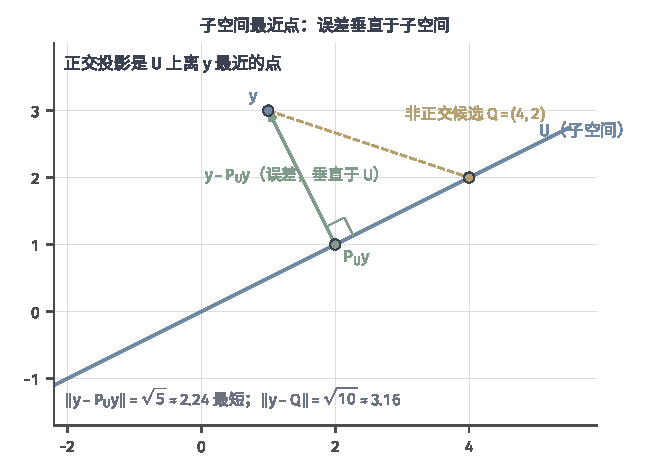
\includegraphics[width=112mm]{figures/00-shared/mathematical-preliminaries-upper/02-linear-spaces/matplotlib/ls-orthogonal-projection-nearest/ls-orthogonal-projection-nearest.pdf}
  \caption{直线子空间$U$（过原点、方向$(2,1)$）上离$\bm y=(1,3)^\top$最近的点是正交投影
  $\bm p=(2,1)^\top$，误差$\bm y-\bm p=(-1,2)^\top$与$U$垂直（直角小方块）；
  同一线上的另一候选$\bm q=(4,2)^\top$到$\bm y$的距离$\sqrt{10}$明显大于最短距离$\sqrt5$。
  这是解析式教学构造。}
  \label{fig:ls-orthogonal-projection-nearest}
\end{figure}

\paragraph{正规方程}

回到矩阵$\bm A$，取$U=\operatorname{range}(\bm A)$，设最近点是$\hat{\bm b}=\bm A\hat{\bm x}$。
列空间由$\bm A$的各列张成，残差$\bm r=\bm b-\bm A\hat{\bm x}$与列空间正交，就是与每一列$\bm a_j$正交，
即$\bm a_j^\top\bm r=0$，$j=1,\ldots,d$，合写为$\bm A^\top\bm r=\bm0$。代入$\bm r$得到\term{正规方程}（normal equations）
\begin{equation}
\begin{gathered}
\bm A^\top(\bm b-\bm A\hat{\bm x})=\bm0\\
\bm A^\top\bm A\hat{\bm x}=\bm A^\top\bm b.
\end{gathered}
\label{eq:linear-algebra-normal-equations}
\end{equation}
“正规”指法向，即残差与列空间正交，不是归一化。由定理~\ref{thm:ls-four-subspaces-orthogonality}，
这也就是说残差落在左零空间$\operatorname{null}(\bm A^\top)$中：最小二乘把$\bm b$分成可达的部分与完全不可达的部分。
下面用一个三个方程、两个未知量的例子计算正规方程。

\begin{example}[超定方程的最小二乘解]
\label{ex:ls-normal-equations-three-by-two}
取$\bm A=\left[\begin{smallmatrix}1&0\\0&1\\1&1\end{smallmatrix}\right]$、$\bm b=(2,3,2)^\top$。
列空间中的向量形如$(x_1,x_2,x_1+x_2)^\top$，第三坐标等于前两坐标之和；而$\bm b$的第三坐标$2\neq2+3$，
所以$\bm b$不在列空间中，方程$\bm A\bm x=\bm b$无解。计算
\[
\begin{gathered}
\bm A^\top\bm A=\begin{bmatrix}2&1\\1&2\end{bmatrix}\\
\bm A^\top\bm b=\begin{bmatrix}4\\5\end{bmatrix},
\end{gathered}
\]
解正规方程$2\hat x_1+\hat x_2=4$、$\hat x_1+2\hat x_2=5$，得$\hat{\bm x}=(1,2)^\top$。
最近点为$\bm A\hat{\bm x}=(1,2,3)^\top$，残差为$\bm r=\bm b-\bm A\hat{\bm x}=(1,1,-1)^\top$；
它与两列$(1,0,1)^\top$、$(0,1,1)^\top$的内积都是零，满足正交性判据。
\end{example}

图~\ref{fig:ls-least-squares-residual}画出这个例子。

\begin{figure}[htbp]
  \centering
  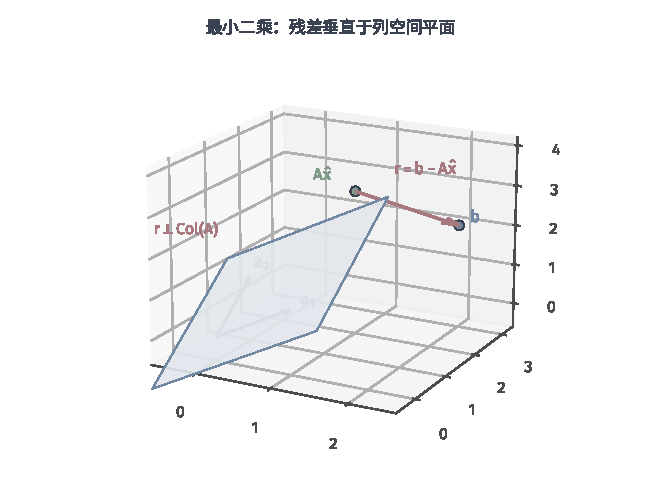
\includegraphics[width=112mm]{figures/00-shared/mathematical-preliminaries-upper/02-linear-spaces/matplotlib/ls-least-squares-residual/ls-least-squares-residual.pdf}
  \caption{列空间平面上的最近点。$\bm A=\left[\begin{smallmatrix}1&0\\0&1\\1&1\end{smallmatrix}\right]$，
  列$\bm a_1=(1,0,1)^\top$、$\bm a_2=(0,1,1)^\top$张成浅蓝平面；$\bm b=(2,3,2)^\top$，
  最近拟合值$\bm A\hat{\bm x}=(1,2,3)^\top$，残差$\bm r=(1,1,-1)^\top$满足
  $\bm r^\top\bm a_1=\bm r^\top\bm a_2=0$。透视教学构造。}
  \label{fig:ls-least-squares-residual}
\end{figure}

正规方程是由几何判据推出的；也可以直接验证，它的解确实使目标取全局最小。

设$\hat{\bm x}$满足正规方程，
$\bm r=\bm b-\bm A\hat{\bm x}$，对任意增量$\bm h$，$\bm A(\hat{\bm x}+\bm h)-\bm b=\bm A\bm h-\bm r$，展开平方长度得
\[
 \lVert\bm A(\hat{\bm x}+\bm h)-\bm b\rVert_2^2
 =\lVert\bm r\rVert_2^2-2(\bm A\bm h)^\top\bm r+\lVert\bm A\bm h\rVert_2^2
 =\lVert\bm r\rVert_2^2-2\bm h^\top(\bm A^\top\bm r)+\lVert\bm A\bm h\rVert_2^2 .
\]
正规方程使中间项为零，剩下的$\lVert\bm A\bm h\rVert_2^2\geq0$，所以任何移动都不会减小目标。
反之，若$\hat{\bm x}$是最小点，则拟合值$\bm A\hat{\bm x}$是列空间中离$\bm b$最近的点，由正交性判据，
残差与列空间正交，$\hat{\bm x}$满足正规方程。于是最小二乘问题与正规方程同解，
求最小点就是解这个$d$阶对称线性方程。

用一般子空间的基矩阵$\bm B$代替$\bm A$，并在一般内积下把$\bm B^\top\bm B$的元素换成内积，正规方程成为
\begin{equation}
\begin{gathered}
\bm G\bm c=\bigl(\langle\bm b_i,\bm y\rangle\bigr)_{i=1}^r\\
g_{i,j}=\langle\bm b_i,\bm b_j\rangle,
\end{gathered}
\label{eq:ls-gram-system}
\end{equation}
系数矩阵$\bm G$是基向量的Gram矩阵；逐行写就是$\sum_j\langle\bm b_i,\bm b_j\rangle c_j=\langle\bm b_i,\bm y\rangle$，
即残差$\bm y-\sum_jc_j\bm b_j$与每个基向量正交。这就把问题~\eqref{eq:ls-nearest-point-coefficients}化成了线性方程。

在示例~\ref{ex:ls-nonorthogonal-coefficients}中，$\bm G=\left[\begin{smallmatrix}2&1\\1&1\end{smallmatrix}\right]$，右端为$(1,0)^\top$，
解得$\bm c=(1,-1)^\top$，与直接观察一致。这里两个基向量张成整个平面，所以最近点就是$\bm y$本身；
Gram系统的作用是把内积$(1,0)^\top$纠正为真正的系数。

基向量标准正交时，Gram矩阵是单位矩阵，Gram系统不必求解：系数就是内积，最近点直接写出，
\[
 \bm p=\sum_j\langle\bm q_j,\bm y\rangle\bm q_j .
\]
这就是第~\ref{chap:normed-inner-product-spaces}章的正交分解公式~\eqref{eq:ls-orthonormal-projection}，每个系数只与自己的方向有关，互不干扰。
它是第~\ref{sec:ls-qr-method}节用QR分解解最小二乘的出发点。

\subsection{解的存在与唯一性}
\label{sec:ls-ls-existence}

最近点$\hat{\bm b}$作为列空间中的点总是存在且唯一，但正规方程的未知量是产生它的输入$\hat{\bm x}$。
本部分回答：这样的输入是否总存在，是否唯一，不唯一时全部解是什么样子，唯一时系数是否可靠。

\paragraph{存在性}

正规方程对任意$\bm b$都有解。几何上这很自然：$\hat{\bm b}$在列空间中，总有输入产生它，而这个输入满足正规方程。
也可以从方程本身验证。先看系数矩阵的零空间：若$\bm A^\top\bm A\bm x=\bm0$，则
$\lVert\bm A\bm x\rVert_2^2=\bm x^\top\bm A^\top\bm A\bm x=0$，即$\bm A\bm x=\bm0$；反向包含显然。故
\begin{equation}
 \ker(\bm A^\top\bm A)=\ker\bm A.
 \label{eq:ls-normal-kernel}
\end{equation}
由定理~\ref{thm:ls-four-subspaces-orthogonality}，对任意矩阵有$\operatorname{range}(\bm A^\top)=(\ker\bm A)^\perp$。把它用在对称矩阵$\bm A^\top\bm A$上，得
$\operatorname{range}(\bm A^\top\bm A)=\ker(\bm A^\top\bm A)^\perp=(\ker\bm A)^\perp=\operatorname{range}(\bm A^\top)$。
右端$\bm A^\top\bm b$显然在$\operatorname{range}(\bm A^\top)$中，所以方程总是相容。

\paragraph{全部解与唯一性}

拟合值唯一，不代表输入唯一。正规方程是相容的线性方程，按第~\ref{sec:ls-uniqueness-freedom}节的结论，它的全部解是一个解加上系数矩阵的零空间；
由~\eqref{eq:ls-normal-kernel}，全部解为
\begin{equation}
 \hat{\bm x}+\ker\bm A.
 \label{eq:ls-all-ordinary-solutions}
\end{equation}
这些解给出同一个拟合值，因为零空间方向不改变输出。于是解唯一当且仅当$\bm A$满列秩。
此时$\bm A^\top\bm A$正定（$\bm x\neq\bm0$时$\bm x^\top\bm A^\top\bm A\bm x=\lVert\bm A\bm x\rVert_2^2>0$），因而可逆，唯一解为
\begin{equation}
 \hat{\bm x}=(\bm A^\top\bm A)^{-1}\bm A^\top\bm b.
 \label{eq:linear-algebra-full-rank-least-squares}
\end{equation}
用子空间的基表示时同样如此：基向量线性无关，Gram矩阵$\bm G$正定，Gram系统~\eqref{eq:ls-gram-system}的解唯一。

这里有两层唯一性要分清。最近点作为$U$中的点总是唯一的；它的系数只在张成向量线性无关时唯一：
若$\bm B\bm c_1=\bm B\bm c_2$，则$\bm B(\bm c_1-\bm c_2)=\bm0$，线性无关迫使$\bm c_1=\bm c_2$。

秩亏时，例如$\bm A$有两列相同，正规方程相容但有无穷多解，第~\ref{sec:ls-select-among-solutions}节的讨论原样适用：
若要求欧氏范数最小，就去掉不改变输出的零空间分量，所得的解落在$(\ker\bm A)^\perp$中，
它也是相容方程$\bm A\bm x=\hat{\bm b}$的最小范数解。
在任意秩下把这一选择写成矩阵需要伪逆，见第~\ref{sec:ls-pseudoinverse}节。

无论解是否唯一，最小值都只由正交分解决定。$\hat{\bm b}\perp\bm r$，勾股恒等式给出
$\lVert\bm b\rVert_2^2=\lVert\hat{\bm b}\rVert_2^2+\lVert\bm r\rVert_2^2$：
观测的平方长度分成被列空间解释的部分与残差部分，最小平方残差
$\lVert\bm r\rVert_2^2=\lVert\bm b\rVert_2^2-\lVert\hat{\bm b}\rVert_2^2$对全部解相同。
示例~\ref{ex:ls-normal-equations-three-by-two}中，$\lVert\bm b\rVert_2^2=17$，$\lVert\hat{\bm b}\rVert_2^2=1+4+9=14$，$\lVert\bm r\rVert_2^2=3$。

\paragraph{唯一不等于稳定}

满列秩只保证系数唯一，不保证系数可靠。下面的例子中，设计矩阵的两列接近共线。

\begin{example}[近共线设计：唯一但不稳定的系数]
\label{ex:ls-nearly-collinear-design}
取互相正交的向量$\bm c_1=(1,1,1)^\top$与$\bm q=(0,1,-1)^\top$。
设计矩阵$\bm X_\varepsilon$的两列为$\bm c_1$与$\bm c_1+\varepsilon\bm q$，响应为$\bm y=\bm c_1+\delta\bm q$。
利用$\bm c_1^\top\bm q=0$、$\lVert\bm c_1\rVert_2^2=3$、$\lVert\bm q\rVert_2^2=2$，正规方程为
\[
 \begin{bmatrix}3&3\\3&3+2\varepsilon^2\end{bmatrix}\hat{\bm w}
 =\begin{bmatrix}3\\3+2\varepsilon\delta\end{bmatrix},
\]
系数矩阵的行列式为$6\varepsilon^2$。$\varepsilon\neq0$时满列秩，解为
\begin{equation}
\begin{gathered}
\hat{\bm w}_\varepsilon
 =\begin{bmatrix}1-\delta/\varepsilon\\\delta/\varepsilon\end{bmatrix}\\
\bm X_\varepsilon\hat{\bm w}_\varepsilon=\bm y,
\end{gathered}
\label{eq:linear-algebra-nearly-collinear-least-squares}
\end{equation}
后一式可直接验证：$(1-\delta/\varepsilon)\bm c_1+(\delta/\varepsilon)(\bm c_1+\varepsilon\bm q)=\bm c_1+\delta\bm q$。
取$\varepsilon=0.01$、$\delta=0.1$，系数为$(-9,10)^\top$，残差却为零。

$\varepsilon=0$时两列重合为$\bm c_1$。此时$\bm y=\bm c_1+\delta\bm q$本身就是正交分解，最近输出为$\bm c_1$，
残差为$\delta\bm q$，平方残差为$2\delta^2$；满足$w_1+w_2=1$的系数都是解。
\end{example}

所以$\delta\neq0$时，随着$\varepsilon\to0$，精确拟合所需的系数趋于无穷，而极限矩阵已经不能精确拟合。
拟合值可以相当稳定，表示它的两个系数却可能很大，而且对$\varepsilon$、$\delta$极为敏感。
这是近共线几何本身的性质，不是计算机舍入造成的；它的定量刻画见第~\ref{sec:ls-ordinary-ls-sensitivity}节。

\subsection{正规方程法}
\label{sec:ls-normal-equations-method}

本小节的输入仍是$\bm A\in\mathbb R^{m\times d}$与$\bm b\in\mathbb R^m$，这里假设$m\geq d$且$\bm A$满列秩。原方程可能不相容，因此输出改为唯一的最小二乘解$\hat{\bm x}$。

上一小节已经把最优性写成$\bm A^\top(\bm b-\bm A\hat{\bm x})=0$；正规方程法直接把这个条件当作待求解的$d$阶正定方程。

最直接的算法是解正规方程。$\bm A$满列秩时$\bm A^\top\bm A$对称正定，可以用Cholesky分解：
先形成$\bm A^\top\bm A$与$\bm A^\top\bm b$，分解$\bm A^\top\bm A=\bm L\bm L^\top$，再依次前代解$\bm L\bm z=\bm A^\top\bm b$、
回代解$\bm L^\top\hat{\bm x}=\bm z$。加权问题对$\bm A^\top\bm M\bm A$作同样的分解。
稠密情形下，形成$\bm A^\top\bm A$约需$md^2$次乘法，分解约需$d^3/3$次运算，多个右端复用同一分解。
$m$远大于$d$且矩阵条件良好时，形成正规矩阵再作Cholesky分解，通常比稠密QR所需运算更少。

例如仍用$\bm A=\left[\begin{smallmatrix}1&0\\0&1\\1&1\end{smallmatrix}\right]$和$\bm b=(2,3,2)^\top$。先算出
\[
 \bm G=\bm A^\top\bm A=\begin{bmatrix}2&1\\1&2\end{bmatrix},\qquad
 \bm c=\bm A^\top\bm b=\begin{bmatrix}4\\5\end{bmatrix}.
\]
Cholesky因子为$\bm L=\left[\begin{smallmatrix}\sqrt2&0\\1/\sqrt2&\sqrt{3/2}\end{smallmatrix}\right]$。前代$\bm L\bm z=\bm c$得到$\bm z=(2\sqrt2,\sqrt6)^\top$，回代$\bm L^\top\hat{\bm x}=\bm z$得到$\hat{\bm x}=(1,2)^\top$。原残差为$(1,1,-1)^\top$，虽非零，却满足$\bm A^\top\bm r=0$，这才是最小二乘计算要核验的条件。

形成$\bm A^\top\bm A$会损失精度。由第~\ref{sec:ls-svd}节的奇异值分解，$\bm A^\top\bm A$的特征值是$\bm A$的奇异值的平方：
$\bm A$中被压缩得很厉害的方向，在$\bm A^\top\bm A$中被压缩两次，就像一个小数取平方后更小；
浮点计算中，这种方向可能与零无法区分。所以正规方程法只在各列明显线性无关、
$\bm A^\top\bm A$的正定性有充足余量时可靠。秩亏时唯一性本身就不成立；近秩亏时，如示例~\ref{ex:ls-nearly-collinear-design}，
系数本来就不稳定，Cholesky分解成功也不说明结果可用。这种平方造成的精度损失在第~\ref{sec:ls-numerical-sensitivity}节用条件数定量估计。

\subsection{QR分解}
\label{sec:ls-qr-method}
\label{sec:linear-algebra-direct-residual}

另一条路线不形成$\bm A^\top\bm A$，而是先给列空间换一组标准正交基。
第~\ref{chap:normed-inner-product-spaces}章的Gram--Schmidt正交化正是做这件事，它把满列秩矩阵写成经济型QR分解
$\bm A=\bm Q\bm R$（式~\eqref{eq:ls-qr-factorization}），$\bm Q$的列是列空间的标准正交基，$\bm R$是对角元为正的上三角矩阵。
QR适合最小二乘的根本原因是：正交矩阵保持欧氏长度，用它变换残差，只改坐标，不改长度，最小点也就不变。

设$\bm A$满列秩，把$\bm Q$的列扩充成$\mathbb R^m$的标准正交基，得到完全QR分解
$\bm A=[\bm Q_1\;\bm Q_2]\left[\begin{smallmatrix}\bm R\\\bm0\end{smallmatrix}\right]=\bm Q_1\bm R$，
其中$[\bm Q_1\;\bm Q_2]$是$m$阶正交矩阵，$\bm Q_1$有$d$列，就是经济型分解中的$\bm Q$；$\bm Q_2$的列张成列空间的正交补。
记$\bm c_1=\bm Q_1^\top\bm b$、$\bm c_2=\bm Q_2^\top\bm b$。用$[\bm Q_1\;\bm Q_2]^\top$变换残差，
\[
 \lVert\bm A\bm x-\bm b\rVert_2^2
 =\left\lVert\begin{bmatrix}\bm R\bm x-\bm c_1\\-\bm c_2\end{bmatrix}\right\rVert_2^2
 =\lVert\bm R\bm x-\bm c_1\rVert_2^2+\lVert\bm c_2\rVert_2^2 .
\]
第二项与$\bm x$无关，是无法消除的残差；第一项可以通过解上三角方程$\bm R\hat{\bm x}=\bm c_1$降为零。
满列秩时$\bm R$的对角元非零，回代即得唯一解，最小平方残差就是$\lVert\bm c_2\rVert_2^2=\lVert\bm b\rVert_2^2-\lVert\bm c_1\rVert_2^2$，
所以$\bm Q_2$不必形成。整个过程不出现$\bm A^\top\bm A$，避免了正规方程法的平方尺度损失，
代价是分解的运算量高于Cholesky。

下面用QR分解重算示例~\ref{ex:ls-normal-equations-three-by-two}。

\begin{example}[用QR分解求解最小二乘]
\label{ex:ls-qr-three-by-two}
仍取$\bm A=\left[\begin{smallmatrix}1&0\\0&1\\1&1\end{smallmatrix}\right]$、$\bm b=(2,3,2)^\top$。
Gram--Schmidt先给出$\bm q_1=(1,0,1)^\top/\sqrt2$。$\bm a_2$在$\bm q_1$上的分量为$r_{1,2}=\bm q_1^\top\bm a_2=1/\sqrt2$，扣除后
\[
 \begin{gathered}
\bm v_2=(0,1,1)^\top-\tfrac12(1,0,1)^\top=(-\tfrac12,1,\tfrac12)^\top\\
r_{2,2}=\lVert\bm v_2\rVert_2=\sqrt{3/2},
 \end{gathered}
\]
再令$\bm q_2=\bm v_2/r_{2,2}$。于是
\[
\begin{gathered}
\bm R=\begin{bmatrix}\sqrt2&1/\sqrt2\\0&\sqrt{3/2}\end{bmatrix}\\
\bm c_1=\begin{bmatrix}\bm q_1^\top\bm b\\\bm q_2^\top\bm b\end{bmatrix}=\begin{bmatrix}2\sqrt2\\\sqrt6\end{bmatrix}.
\end{gathered}
\]
回代解$\bm R\hat{\bm x}=\bm c_1$，得$\hat x_2=\sqrt6/\sqrt{3/2}=2$、$\hat x_1=(2\sqrt2-2/\sqrt2)/\sqrt2=1$，
与正规方程的结果相同。最小平方残差为$\lVert\bm b\rVert_2^2-\lVert\bm c_1\rVert_2^2=17-(8+6)=3$，也与前面一致。
\end{example}

同一分解还给出最近点。最近点为$\hat{\bm b}=\bm A\hat{\bm x}=\bm Q_1\bm R\hat{\bm x}=\bm Q_1\bm c_1=\bm Q_1\bm Q_1^\top\bm b$，
$\bm c_1$的分量就是$\bm b$在各正交方向上的坐标，不必另解Gram系统。

它也判定相容性：$\bm c_2=\bm0$当且仅当$\bm b$在列空间中，
此时回代得到的就是原方程的精确解；$\bm c_2\neq\bm0$时原方程不相容，$\lVert\bm c_2\rVert_2$就是$\bm b$到列空间的距离。
例如$\bm A=\left[\begin{smallmatrix}1&1\\1&0\\0&1\end{smallmatrix}\right]$、$\bm b=(2,1,1)^\top=\bm A(1,1)^\top$时$\bm c_2=\bm0$，
回代得到精确解$\hat{\bm x}=(1,1)^\top$。这就是第~\ref{sec:ls-direct-methods}节所说的：
超定而满列秩的方程，相容性的判断与唯一解的计算可以由同一个QR分解一次完成。

$\bm A$秩亏时，Gram--Schmidt在某一列得不到新方向，$\bm R$不再可逆，上面的回代不能直接进行；
这时最小二乘解不唯一，最小范数解由第~\ref{sec:ls-pseudoinverse}节的伪逆给出。
有限精度下怎样借带列主元的QR判断秩，见第~\ref{sec:ls-orthogonalization-qr}节。

\paragraph{列空间投影与正规方程}

不做正交化，也可以从正规方程写出投影矩阵。$\bm A$满列秩时，最近点为
$\hat{\bm b}=\bm A\hat{\bm x}=\bm A(\bm A^\top\bm A)^{-1}\bm A^\top\bm b$，故
\begin{equation}
 \bm P_{\operatorname{range}(\bm A)}=\bm A(\bm A^\top\bm A)^{-1}\bm A^\top.
 \label{eq:ls-column-space-projector}
\end{equation}
直接相乘可验它对称且幂等。代入$\bm A=\bm Q\bm R$，得$\bm Q\bm R(\bm R^\top\bm R)^{-1}\bm R^\top\bm Q^\top=\bm Q\bm Q^\top$，
与式~\eqref{eq:linear-algebra-orthogonal-projector}一致，说明投影只取决于列空间，与所用的基无关。

回归中这个矩阵常称帽子矩阵，它把观测$\bm y$映成拟合值$\hat{\bm y}$；$\bm I-\bm P$则把观测映成残差，
它是到$\operatorname{range}(\bm A)^\perp=\operatorname{null}(\bm A^\top)$的正交投影。
加权内积下，同样的推导给出$\bm A(\bm A^\top\bm M\bm A)^{-1}\bm A^\top\bm M$；它幂等但一般不对称，
在普通内积下是斜投影，在$\bm M$内积下才是正交投影。

两个正交投影相乘一般不可交换，$\bm P_U\bm P_V\neq\bm P_V\bm P_U$，乘积也未必还是投影。
两者可交换时，乘积既幂等又对称，因而是到其像的正交投影。它的像含于$U$（左因子是$\bm P_U$），
也含于$V$（交换次序后左因子是$\bm P_V$），而$U\cap V$中的向量被它保持不变，所以它是到$U\cap V$的正交投影。


\subsection{修正Gram--Schmidt正交化}

上面已经说明如何用QR分解把最小二乘化为三角方程，现在还需说明分解本身怎样计算。
第~\ref{chap:normed-inner-product-spaces}章用Gram--Schmidt正交化构造它，那里假定精确算术：
式~\eqref{eq:ls-gram-schmidt}一次性减去$\bm a_j$在全部旧方向上的分量，每个系数都用原始的$\bm a_j$计算。

\term{修正Gram--Schmidt}（modified Gram--Schmidt）改为逐个扣除：先令$\bm u\leftarrow\bm a_j$，对$i=1,\ldots,j-1$依次计算$r_{i,j}=\langle\bm u,\bm q_i\rangle$并更新$\bm u\leftarrow\bm u-r_{i,j}\bm q_i$，最后归一化。

具体说，第$j$列处理结束后，令$r_{j,j}=\|\bm u\|_2$、$\bm q_j=\bm u/r_{j,j}$；若该范数为零，当前列不能提供新方向，应转入秩亏处理。对$j=1,\ldots,d$重复，输出$\bm Q=[\bm q_1\;\cdots\;\bm q_d]$与$\bm R=(r_{i,j})$。

随后计算$c_j=\bm q_j^\top\bm b$并回代$\bm R\hat{\bm x}=\bm c$，才完成输入$(\bm A,\bm b)$到最小二乘解的过程。前面的三行两列算例中，第二列只有一个旧方向可扣除，按这一流程同样得到$\hat{\bm x}=(1,2)^\top$。

精确算术中两种做法给出同样的结果：扣除第$i$个方向时，此前已减去的都是$\bm q_1,\ldots,\bm q_{i-1}$的倍数，它们与$\bm q_i$正交，所以$\langle\bm u,\bm q_i\rangle=\langle\bm a_j,\bm q_i\rangle$。

有限精度下，修正的做法每次都从已经扣除过的最新残差出发，算出的$\bm q_j$之间正交性的损失通常更小；
它的损失大致与$\kappa_2(\bm A)$乘单位舍入$u$同量级，原始做法则可能严重得多\scite{math-golub2013matrix}。
列之间越接近线性相关，扣除后剩下的$\bm u_j$越短，舍入误差在其中所占的比例越大，两种做法的差别也越明显。

同样的原因使列相关时的处理不能照搬精确算术：有限精度下$\bm u_j$很少恰好为零，判断“没有新方向”时要把$\lVert\bm u_j\rVert$与一个容限比较，
这正是第~\ref{sec:ls-ordinary-ls-sensitivity}节的数值秩问题。修正Gram--Schmidt的正交性损失仍随条件数增长；
需要$\bm Q$在工作精度下正交时，改用后面的Householder反射。

\subsection{Householder反射}
\label{sec:ls-orthogonalization-qr}

修正Gram--Schmidt仍从列出发构造$\bm Q$，列越接近线性相关，正交性损失越大，而这恰是最需要QR的情形。
稠密计算中更常用的做法反过来：用一串正交矩阵从左边作用于$\bm A$，逐列把主对角线以下的元素消成零，最后剩下上三角的$\bm R$。
正交矩阵保持长度，这样的消元不会放大误差，各步正交矩阵的乘积自然是正交的。
完成这一步的基本工具是\term{Householder反射}，它一次消去一列中主对角线以下的全部元素。

对非零向量$\bm a$，要找一个正交矩阵把它变成$\bm e_1$的倍数。由于正交变换保持长度，目标只能是$\pm\lVert\bm a\rVert_2\bm e_1$。
取$s=1$（若$a_1\geq0$）或$s=-1$（若$a_1<0$），令
\begin{equation}
\begin{gathered}
\bm v=\bm a+s\lVert\bm a\rVert_2\bm e_1\\
\bm H=\bm I-2\frac{\bm v\bm v^\top}{\bm v^\top\bm v}.
\end{gathered}
\label{eq:ls-householder}
\end{equation}
$\bm H$把$\bm v$方向的分量变号，与$\bm v$正交的分量保持不变，即关于以$\bm v$为法向的超平面作镜面反射；
它对称，且$\bm H^\top\bm H=\bm H^2=\bm I$，反射两次回到原处。

下面验证它把$\bm a$送到$\bm e_1$方向。记$\alpha=\lVert\bm a\rVert_2$，则
$\bm v^\top\bm a=\alpha^2+s\alpha a_1$，$\bm v^\top\bm v=\alpha^2+2s\alpha a_1+\alpha^2=2\bm v^\top\bm a$，于是
\[
 \bm H\bm a=\bm a-2\frac{\bm v^\top\bm a}{\bm v^\top\bm v}\bm v=\bm a-\bm v=-s\alpha\bm e_1 .
\]
符号$s$取与$a_1$相同，是为了让$\bm v$的首元素$a_1+s\alpha$是两个同号数相加，避免两个相近的数相减而丢失有效数字。
应用$\bm H$时只需保存$\bm v$，计算$\bm H\bm x=\bm x-2\bm v(\bm v^\top\bm x)/(\bm v^\top\bm v)$，不必形成整个矩阵。

\begin{example}[二维向量的Householder反射]
\label{ex:ls-householder-two-dim}
取$\bm a=(3,4)^\top$。$a_1>0$，取$s=1$；$\alpha=5$，$\bm v=\bm a+5\bm e_1=(8,4)^\top$，$\bm v^\top\bm v=80$。于是
\[
 \bm H=\bm I-\frac{2}{80}\bm v\bm v^\top
 =\bm I-\frac1{40}\begin{bmatrix}64&32\\32&16\end{bmatrix}
 =\begin{bmatrix}-3/5&-4/5\\-4/5&3/5\end{bmatrix},
\]
$\bm H\bm a=(-5,0)^\top$，与$-s\alpha\bm e_1=-5\bm e_1$一致。
\end{example}

对矩阵做QR时，第$k$步对第$k$列从第$k$个元素往下的部分构造反射，
只作用于尚未处理的右下子块。$d$步之后，$\bm H_d\cdots\bm H_1\bm A=\left[\begin{smallmatrix}\bm R\\\bm0\end{smallmatrix}\right]$，
各反射的乘积的转置就是完全QR分解中的$[\bm Q_1\;\bm Q_2]$；
$\bm R$的对角元可能为负，把相应的行与$\bm Q_1$的列同时变号即可化为对角元为正的形式。

把这一过程用于求解时，令工作矩阵$\bm F=\bm A$、工作右端$\bm c=\bm b$。第$k$步用$\bm F_{k:m,k}$构造反射，把它同时作用于$\bm F_{k:m,k:d}$与$\bm c_{k:m}$；前面已经消出的零不再改变。全部列处理完后，$\bm F$的前$d$行是$\bm R$，$\bm c$的前$d$项是$\bm c_1$，回代得到$\hat{\bm x}$，其余项组成不可消除的残差坐标$\bm c_2$。

若为统一符号而翻转$\bm R$某行，也须同步翻转$\bm c_1$的对应项。

例如取$\bm A=\left[\begin{smallmatrix}3&1\\4&2\end{smallmatrix}\right]$、$\bm b=(4,6)^\top$。用上例的反射同时变换二者，得到
\[
 \bm H\bm A=\begin{bmatrix}-5&-11/5\\0&2/5\end{bmatrix},\qquad
 \bm H\bm b=\begin{bmatrix}-36/5\\2/5\end{bmatrix}.
\]
由第二行得$x_2=1$，再由第一行得$x_1=1$。反射后的矩阵已经是上三角形，因而本例无需继续消元；代回可验$\bm A\bm x=\bm b$。

稠密$m\times d$矩阵的Householder QR约需$2md^2-2d^3/3$次浮点运算。$\bm Q$不必显式形成，
保存各步的反射向量即可；求解最小二乘时，把同样的反射依次作用于$\bm b$就得到$\bm c_1$与$\bm c_2$，
多个右端复用全部反射与$\bm R$。岭回归对堆叠矩阵~\eqref{eq:ls-augmented-system}作同样的分解即可，
不必形成$\bm A^\top\bm A+\lambda\bm L^\top\bm L$。

秩亏或接近秩亏时，要先把列重新排序。带列主元的QR在每一步选剩余部分中最长的一列先处理，
使接近零的对角元集中在$\bm R$的尾部，从而暴露数值秩，阈值按数据误差的尺度选取，这比计算奇异值分解便宜。
若精确秩为$r$，只用前$r$个主元列回代、其余未知量取零，得到的基本解使原目标达到最小，
但一般不是最小范数解，正如第~\ref{sec:ls-select-among-solutions}节中自由变量取零得到的特解一般不是最小范数解。若$r$由数值阈值确定，被忽略的方向未必精确为零，此时得到的是截断近似，不能保证它是原问题的精确最小二乘解。

\subsection{Givens旋转}

Householder一次处理整段列向量；当只需消去少数元素，或者新观测只增加了一行时，重新反射整个子块可能不划算。Givens方法只混合两行，同步更新这两行的系数与右端，仍以得到三角方程并回代为目标。输入输出与Householder求解相同，差别在于每一步消元的范围。

\term{Givens旋转}一次只消去一个元素。它在第$i$、$j$两个坐标构成的平面内作旋转，其余坐标不变；
在这两个坐标上的作用是
\begin{equation}
\begin{gathered}
\begin{bmatrix}a_i\\a_j\end{bmatrix}\mapsto
 \begin{bmatrix}c&s\\-s&c\end{bmatrix}
 \begin{bmatrix}a_i\\a_j\end{bmatrix}\\
c^2+s^2=1.
\end{gathered}
\label{eq:ls-givens}
\end{equation}
这里的$c$、$s$是旋转角的余弦与正弦，与Householder反射中的符号$s$无关。
完整的矩阵$\bm G(i,j)$是在单位矩阵的$(i,i),(i,j),(j,i),(j,j)$四个位置放上$c,s,-s,c$。
为了消去$a_j$，取$r=\sqrt{a_i^2+a_j^2}$，$c=a_i/r$、$s=a_j/r$，则新分量为
$(ca_i+sa_j,\,-sa_i+ca_j)=(r,0)$。$r=0$时两个分量本已为零，无需旋转。

\begin{example}[二维向量的Givens旋转]
\label{ex:ls-givens-two-dim}
取$(a_i,a_j)=(3,4)$。$r=\sqrt{9+16}=5$，$c=3/5$、$s=4/5$，旋转后
\[
 \begin{gathered}
ca_i+sa_j=\frac95+\frac{16}5=5\\
-sa_i+ca_j=-\frac{12}5+\frac{12}5=0 ,
 \end{gathered}
\]
第二个分量被消去，长度$5$全部转到第一个分量上。
\end{example}

对一般$m\times d$的输入，先令$\bm F=\bm A$、$\bm c=\bm b$。按列$k=1,\ldots,d$处理，每列从底部$i=m$向上到$k+1$，对当前的$f_{i-1,k},f_{i,k}$构造旋转，混合第$i-1,i$行的第$k$至$d$列，并同步混合$c_{i-1},c_i$。这样逐个把对角线以下的元素消为零，而且不会破坏前面列中的零。最后取前$d$行得到$\bm R$，回代$\bm R\hat{\bm x}=\bm c_{1:d}$。

在上一小节同一个二阶方程中，旋转矩阵取$\bm G=\left[\begin{smallmatrix}3/5&4/5\\-4/5&3/5\end{smallmatrix}\right]$，得到$\bm G\bm A=\left[\begin{smallmatrix}5&11/5\\0&2/5\end{smallmatrix}\right]$与$\bm G\bm b=(36/5,2/5)^\top$。回代仍得$(1,1)^\top$。两种正交变换的中间符号不同，最终求解的是同一个原方程。

Givens每次只改动两行，适合稀疏或带状矩阵，也适合在最小二乘中新增一条观测时逐步更新已有的QR；
对稠密矩阵，它消去同样多的元素需要更多运算，不如Householder。
图~\ref{fig:ls-givens-householder-elimination}把两种变换并置。图中的反射取另一种符号，
把向量映到$(r,0)^\top$而不是$(-r,0)^\top$，精确算术中两种选择都可以。

\begin{figure*}[htbp]
  \centering
  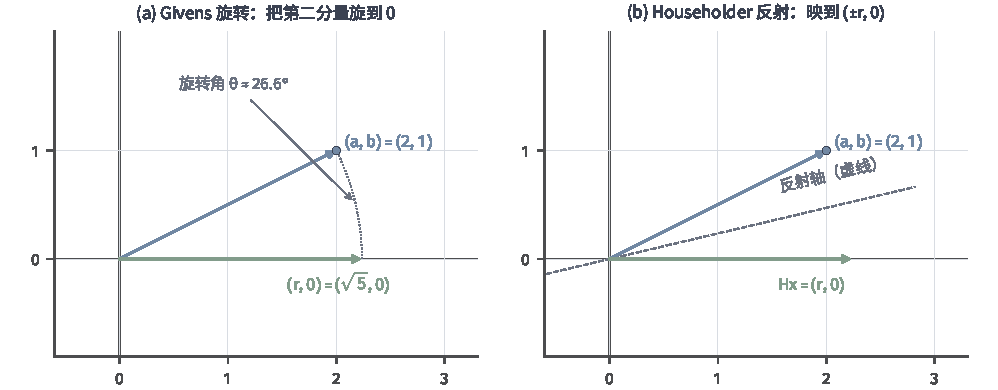
\includegraphics[width=168.998mm]{figures/00-shared/mathematical-preliminaries-upper/02-linear-spaces/matplotlib/ls-givens-householder-elimination/ls-givens-householder-elimination.pdf}
  \caption{两种初等正交消元。左：Givens旋转把$(a,b)=(2,1)^\top$沿圆弧旋到
  $(r,0)^\top$，$r=\sqrt5$，旋转角$\theta=\arctan(1/2)$；右：Householder反射沿角平分线
  把同一向量映到$(r,0)^\top$。两者都是正交变换，保持长度，区别在旋转（行列式$+1$）与
  反射（对称正交）。解析式教学构造。}
  \label{fig:ls-givens-householder-elimination}
\end{figure*}

至此，正规方程与QR都给出了完整的直接求解过程：前者形成正定系统，后者把系数和右端一起作正交变换，再解三角方程。当矩阵很大、无法方便地保存这些因子时，下一组方法用矩阵向量乘法逐步构造小问题。
% LSMR recursion checked against Fong and Saunders, SIAM J. Sci. Comput. 33 (2011), Algorithm LSMR.
% Extended Kaczmarz uses the synchronous old-z update of Zouzias and Freris, arXiv:1205.5770, Algorithm 3.
\subsection{Golub--Kahan双对角化}
\label{sec:ls-bidiagonal-iteration}

前面的QR方法适合能够保存分解结果的问题。若$\bm A\in\mathbb R^{m\times d}$很大，或者只能够计算$\bm A\bm v$与$\bm A^\top\bm u$，可以逐步构造低维问题，每一步只使用这两种乘法。下面从零初值说明；非零初值可以先以$\bm b-\bm A\bm x_0$为右端项求修正，但还要单独检查所得解的零空间分量。

以下统一输入$\bm A,\bm b$、两种残差的容差与最大步数，初值固定为$\bm x_0=0$。LSQR与LSMR的最终输出都是$d$维近似解，区别是每个子空间中优化哪一种残差。双对角化只是二者共享的准备过程：它输出基向量及双对角系数，还没有给出近似解。

为什么要交替使用$\bm A$与$\bm A^\top$？$\bm A$把$d$维未知量送入$m$维观测空间，而最优性条件$\bm A^\top\bm r=0$又把观测残差送回未知量空间。分别在两个空间中保持正交基，就能用很少的系数记录这两个作用，并把大问题的残差精确地表示成小问题的残差。

若$\bm b=0$，零向量已是最小范数解。否则令$\beta_1=\lVert\bm b\rVert_2$、$\bm u_1=\bm b/\beta_1$，再计算$\alpha_1=\lVert\bm A^\top\bm u_1\rVert_2$。若$\alpha_1=0$，零向量已满足正规方程。

当$\alpha_1>0$时令$\bm v_1=\bm A^\top\bm u_1/\alpha_1$。Golub--Kahan双对角化按下式交替生成两个空间中的向量：
\begin{align*}
 \bm p&=\bm A\bm v_k-\alpha_k\bm u_k,\\
 \beta_{k+1}&=\lVert\bm p\rVert_2,\\
 \bm u_{k+1}&=\bm p/\beta_{k+1},\\
 \bm q&=\bm A^\top\bm u_{k+1}-\beta_{k+1}\bm v_k,\\
 \alpha_{k+1}&=\lVert\bm q\rVert_2,\\
 \bm v_{k+1}&=\bm q/\alpha_{k+1}.
\end{align*}

待归一化向量为零时，不能执行对应除法。

若$\beta_{k+1}=0$，当前$\bm B_k$的最后一个下对角元已知为零；此时可令后续旋转所需的$\alpha_{k+1}=0$作为终止时的约定，不定义$\bm u_{k+1}$或$\bm v_{k+1}$。若$\beta_{k+1}>0$但$\alpha_{k+1}=0$，则已知$\bm B_k$和该零值，也不定义$\bm v_{k+1}$。

两种情形都先用已生成的系数完成当前小问题及$\bm x_k$的更新，再检查原残差和正规残差，不构造后续不存在的基向量。

减去旧方向的分量使所得向量在精确算术中与已有基正交。

当$\beta_{k+1}>0$时，把已生成的$\bm u_i$和$\bm v_i$分别排成列，得到$\bm A\bm V_k=\bm U_{k+1}\bm B_k$，其中$\bm B_k$的主对角为$\alpha_1,\ldots,\alpha_k$，下对角为$\beta_2,\ldots,\beta_{k+1}$。若$\beta_{k+1}=0$，则去掉$\bm B_k$的全零末行，记剩余方阵为$\widehat{\bm B}_k$，此时使用$\bm A\bm V_k=\bm U_k\widehat{\bm B}_k$，无需构造$\bm u_{k+1}$。

\subsection{LSQR算法}

有了双对角化输出，下一步要决定原变量怎样取值。LSQR把候选解限制在$\operatorname{span}\{\bm v_1,\ldots,\bm v_k\}$中，并在其中最小化原残差。也就是说，输入数据未变，只把每轮需要选择的未知量从$d$个原坐标换成$k$个子空间坐标。

选择$\bm x_k=\bm V_k\bm y$，并利用$\bm b=\beta_1\bm u_1$与已生成的$\bm U$的正交性，原残差范数化为$\lVert\beta_1\bm e_1-\bm B_k\bm y\rVert_2$。末行因$\beta_{k+1}=0$而删去时，改用$\widehat{\bm B}_k$及$k$维的$\bm e_1$，结果相同。LSQR在每一步求解这个小型最小二乘问题；因此精确算术下，随着候选空间扩大，原残差范数不增。实现可以用Givens旋转逐步更新小问题，不必每轮重新分解，也不必形成$\bm A^\top\bm A$。避免形成正规矩阵能减少填充及其形成误差，却不能消除原问题的小奇异值。

具体实现时，可将新一行双对角元素用一次平面旋转消去，并同时更新解。初始化$\bm x_0=\bm0$、$\bm w_1=\bm v_1$、$\bar\rho_1=\alpha_1$、$\bar\phi_1=\beta_1$。第$k$轮先做上述双对角化，再依次计算
\begin{align*}
 \rho_k&=\sqrt{\bar\rho_k^2+\beta_{k+1}^2},\\
 c_k&=\bar\rho_k/\rho_k,\\
 s_k&=\beta_{k+1}/\rho_k,\\
 \theta_{k+1}&=s_k\alpha_{k+1},\\
 \bar\rho_{k+1}&=-c_k\alpha_{k+1},\\
 \phi_k&=c_k\bar\phi_k,\quad \bar\phi_{k+1}=s_k\bar\phi_k,
\end{align*}
并更新$\bm x_k=\bm x_{k-1}+(\phi_k/\rho_k)\bm w_k$与$\bm w_{k+1}=\bm v_{k+1}-(\theta_{k+1}/\rho_k)\bm w_k$。这些标量记录逐次旋转，小问题的解通过方向$\bm w_k$累加到原变量中。

这个累加式可以从回代读出，而无需把它当作独立公式记忆。旋转把双对角小矩阵化为上双对角矩阵，当前对角元是$\rho_k$，与下一列的耦合是$\theta_{k+1}$。把三角求解与$\bm V_k\bm y$合在一起，已消去的耦合由$\bm w_{k+1}=\bm v_{k+1}-(\theta_{k+1}/\rho_k)\bm w_k$记录；当前右端分量$\phi_k$除以$\rho_k$后，沿$\bm w_k$加回原解。因而无需每轮保存全部基再重新回代。

若双对角化在本轮产生零量，将所需的零系数代入当前旋转与$\bm x_k$的更新，再检查残差；此时不需要计算下一方向$\bm w_{k+1}$。若$\rho_k=0$，则不能执行相应除法，应直接处理已构造的小问题并检查所得解。

由于零初值下$\bm x_k$位于$\operatorname{range}(\bm A^\top)$，若迭代达到$\bm A^\top(\bm b-\bm A\bm x_k)=0$，它既是最小二乘解，又与$\operatorname{null}(\bm A)$正交，因而是最小范数解。有限精度下向量可能失去正交性，必要时可重正交化，但这需要额外存储与内积。每轮主要成本是一遍$\bm A$与一遍$\bm A^\top$的乘法；实际停止时既检查原残差，也检查正规残差，避免把不相容问题固有的非零残差误判为失败。

\subsection{LSMR算法}
\label{sec:ls-lsmr}

不相容的最小二乘问题中，原残差一般不能降到零；达到最小二乘解的条件是$\bm A^\top\bm r=\bm0$。LSMR与LSQR使用同一组双对角化向量，但在候选空间中选择使正规残差$\lVert\bm A^\top(\bm b-\bm A\bm x_k)\rVert_2$最小的近似。

当$\beta_{k+1}>0$且$\alpha_{k+1}>0$时，由双对角化关系，$\bm A^\top\bm U_{k+1}=\bm V_k\bm B_k^\top+\alpha_{k+1}\bm v_{k+1}\bm e_{k+1}^\top$。令$\bm x_k=\bm V_k\bm y$，得到
\[
 \bm A^\top(\bm b-\bm A\bm x_k)
 =\bm V_{k+1}\left(\alpha_1\beta_1\bm e_1-
 \begin{bmatrix}\bm B_k^\top\bm B_k\\
 \alpha_{k+1}\beta_{k+1}\bm e_k^\top\end{bmatrix}\bm y\right).
\]

所以可通过一个$(k+1)\times k$的小最小二乘问题选择$\bm y$。若$\alpha_{k+1}=0$而$\beta_{k+1}>0$，省去含$\bm v_{k+1}$的零项，使用已有的$\bm V_k$及小问题的前$k$行。若$\beta_{k+1}=0$，则用$\bm U_k$、$\bm V_k$和$\widehat{\bm B}_k$，正规残差为$\bm V_k(\alpha_1\beta_1\bm e_1-\widehat{\bm B}_k^\top\widehat{\bm B}_k\bm y)$；两种情形都不引入缺失的基向量。

这个矩阵用于解释方法；实际短递推利用双对角化系数和两组旋转，不形成原矩阵的$\bm A^\top\bm A$。候选空间逐步扩大，故精确算术中正规残差范数不增；这不意味着解误差也逐步下降。

具体计算可按下列顺序。

第一组旋转与LSQR一样，先把双对角作用化为三角作用；LSMR还要最小化经过$\bm A^\top$作用的残差，因此再用第二组旋转消去这一作用带来的耦合。下面的带横线标量保存旋转后的系数，$\bm h_k$与$\bar{\bm h}_k$保存将小问题的坐标恢复到原变量时所需的方向。每轮依次完成双对角化、两组旋转和解的更新，不能把某一组旋转单独当作解。

使用上一小节的$\alpha_1,\beta_1,\bm v_1$初始化
\[
 \begin{gathered}
\bar\alpha_1=\alpha_1\\
\bar\zeta_1=\alpha_1\beta_1\\
\rho_0=\bar\rho_0=\bar c_0=1\\
\bar s_0=0\\
\bm h_1=\bm v_1\\
\bar{\bm h}_0=\bm0\\
\bm x_0=\bm0.
 \end{gathered}
\]

每轮先继续双对角化，得到$\beta_{k+1}$、$\alpha_{k+1}$和$\bm v_{k+1}$。第一组旋转消去新出现的下对角元：
\[
 \begin{gathered}
\rho_k=\sqrt{\bar\alpha_k^2+\beta_{k+1}^2}\\
c_k=\frac{\bar\alpha_k}{\rho_k}\\
s_k=\frac{\beta_{k+1}}{\rho_k}\\
\theta_{k+1}=s_k\alpha_{k+1}\\
\bar\alpha_{k+1}=c_k\alpha_{k+1}.
 \end{gathered}
\]

第二组旋转处理正规残差小问题中的耦合。它使用上一轮保存的四个量：$\bar c_{k-1}$、$\bar s_{k-1}$、$\rho_{k-1}$和$\bar\rho_{k-1}$。依次计算
\begin{align*}
 \bar\theta_k&=\bar s_{k-1}\rho_k,\\
 \bar\rho_k&=\sqrt{(\bar c_{k-1}\rho_k)^2+\theta_{k+1}^2},\\
 \bar c_k&=\frac{\bar c_{k-1}\rho_k}{\bar\rho_k},\\
 \bar s_k&=\frac{\theta_{k+1}}{\bar\rho_k},\\
 \zeta_k&=\bar c_k\bar\zeta_k,\\
 \bar\zeta_{k+1}&=-\bar s_k\bar\zeta_k.
\end{align*}

最后更新辅助方向和近似解：
\[
 \begin{gathered}
\bar{\bm h}_k=\bm h_k-\frac{\bar\theta_k\rho_k}{\rho_{k-1}\bar\rho_{k-1}}\bar{\bm h}_{k-1}\\
\bm x_k=\bm x_{k-1}+\frac{\zeta_k}{\rho_k\bar\rho_k}\bar{\bm h}_k\\
\bm h_{k+1}=\bm v_{k+1}-\frac{\theta_{k+1}}{\rho_k}\bm h_k.
 \end{gathered}
\]

双对角化产生零量时，使用已知零系数完成本轮旋转和$\bm x_k$更新，再检查原残差与正规残差；不计算需要缺失基向量的下一方向。旋转或归一化的分母为零时，先直接处理当前小问题并核验所得解，不能把递推失效当成求解成功。无完整重正交化时，每轮仍主要使用一次$\bm A$和一次$\bm A^\top$作用，以及线性规模的工作向量。

例如取
\[
\begin{gathered}
\bm A=\begin{bmatrix}1&0\\0&2\\0&0\end{bmatrix}\\
\bm b=\begin{bmatrix}1\\1\\1\end{bmatrix}\\
\bm x_0=\bm0.
\end{gathered}
\]
双对角化得到$\beta_1=\sqrt3$，前两步的小矩阵约为
\[
\begin{gathered}
\bm B_1=\begin{bmatrix}1.2910\\1.3166\end{bmatrix}\\
\bm B_2=\begin{bmatrix}1.2910&0\\1.3166&0.9115\\0&0.8771\end{bmatrix}.
\end{gathered}
\]

把第一步的旋转和向量也列出，便能核对递推所得解。初始化时$\alpha_1\approx1.2910$、$\bm v_1\approx(0.4472,0.8944)^\top$；双对角化得到$\beta_2\approx1.3166$、$\alpha_2\approx0.9115$和$\bm v_2\approx(-0.8944,0.4472)^\top$。LSQR据此计算
\[
 \begin{gathered}
\rho_1\approx1.8439\\
c_1\approx0.7001\\
s_1\approx0.7140\\
\theta_2\approx0.6508\\
\phi_1\approx1.2127\\
\bar\phi_2\approx1.2367.
 \end{gathered}
\]
将这些数代入解的更新式，得到下文的第一步解。下一步使用的方向为
\[
 \bm w_2\approx(-1.0523,0.1315)^\top.
\]

LSMR第一组旋转使用相同的$\rho_1,c_1,s_1,\theta_2$，但保留$\bar\alpha_2\approx0.6382$。第二组旋转取$\bar\theta_1=0$、$\bar\rho_1\approx1.9554$、$\bar c_1\approx0.9430$、$\bar s_1\approx0.3328$，得到$\zeta_1\approx2.1086$。因为$\bar{\bm h}_1=\bm v_1$，由$\bm x_1=\zeta_1\bar{\bm h}_1/(\rho_1\bar\rho_1)$得到另一组第一步解。这里两种方法各自的带横线标量属于各自的递推，不能混用。

第一步LSQR给出$\bm x_1\approx(0.2941,0.5882)^\top$，原残差与正规残差范数分别约为$1.2367$和$0.7892$；LSMR给出$\bm x_1\approx(0.2615,0.5231)^\top$，两种范数分别约为$1.2440$和$0.7442$。在同一候选直线上，前者取得更小的原残差，后者取得更小的正规残差。

第二步两者都得到$(1,1/2)^\top$，此时正规残差为零，但第三行无法拟合，所以原残差范数仍为$1$。

LSQR侧重原残差，LSMR侧重正规残差，两者在同一步选出的系数可以不同。零初值使它们的近似都留在行空间，若达到最小二乘条件便选出最小范数解；任意初值和右预条件可能改变这一选解准则。数值计算中应重新检查原残差与正规残差，并区分达到容差、停滞、预算耗尽和递推失效。

\subsection{Kaczmarz算法}
\label{sec:ls-kaczmarz}

前两种方法每步都要遍历矩阵来做乘法。如果数据以单行提供，可以把一行方程当作一次修正的依据。这里先要求$\bm A\bm x=\bm b$相容，输入为各行数据、初值及停止参数；一次更新选择一行，一轮则循环访问全部行。输出仍是原方程的近似解，零初值还规定了多解时的最小范数选择。

当方程按行到达，或者一次只方便读取一行时，可以依次把当前近似投影到各行方程上。记第$i$行为$\bm a_i^\top$，若$\bm a_i\ne\bm0$，则
\begin{equation}
 \bm x_{k+1}=\bm x_{k}+
 \frac{b_i-\bm a_i^\top\bm x_{k}}{\lVert\bm a_i\rVert_2^2}\bm a_i.
 \label{eq:ls-kaczmarz-update}
\end{equation}

分子是当前行残差，修正沿超平面的法向量进行。

这一修正可直接从当前行推导：限制新点为$\bm x_k+t\bm a_i$，代入$\bm a_i^\top\bm x=b_i$，得到$t=(b_i-\bm a_i^\top\bm x_k)/\|\bm a_i\|_2^2$。在所有满足该行的点中，法向修正距离当前点最近，因而就是正交投影。

例如取$\bm A=\left[\begin{smallmatrix}1&0\\1&1\end{smallmatrix}\right]$、$\bm b=(1,2)^\top$，从零开始按第一行、第二行循环。第一次投影得$(1,0)^\top$；第二次的行残差为$1$，行向量平方长度为$2$，因此得到$(3/2,1/2)^\top$。下一轮依次得到$(1,1/2)^\top$和$(5/4,3/4)^\top$，逐步接近共同解$(1,1)^\top$。每次投影只保证刚处理的一行成立，是否可以停止仍须检查所有行。

循环访问所有非零行称为循环Kaczmarz法；一次更新只访问该行的非零元素，一轮的工作量约与整个矩阵的非零元素数同阶。

对相容方程，任一共同解都在每个超平面上。投影的勾股关系说明，每次更新到共同解的距离不增；完整循环访问各行时，近似收敛到某个解。零初值的更新始终位于行空间，所以在解不唯一时得到最小欧氏范数解。

若初值含零空间分量，该分量不会被行投影改变。零行若对应右端零可跳过；右端非零则表明方程不相容，不能执行除零更新。

循环收敛还需要把单步距离不增加强为整轮收缩。固定与初值具有相同零空间分量的共同解，误差始终位于行空间。每次正交投影若不减少误差长度，说明误差已与该行法向正交；一整轮均不减少，就意味着误差属于所有行的共同零空间。在行空间中，这只能是零向量。

因此一轮误差映射在行空间单位球面上处处严格缩短长度。该球面紧且映射连续，最大的长度比小于一，重复完整循环便收敛到零。这补足了从单步投影性质到整个算法收敛的论证；只知道距离单调不增，并不能直接得到方程残差趋于零。

不相容时，逐行投影未必得到最小二乘解。例如$\bm A=(1,1)^\top$、$\bm b=(0,1)^\top$，循环投影使$x$在$0$与$1$之间来回，而最小二乘解为$1/2$。固定步长的循环行投影因此不能一般地求解不相容最小二乘。下面介绍一种扩展方法：估计右端在列空间正交补上的分量，再修正行方程的右端。

\subsection{扩展Kaczmarz算法}

不相容时不存在共同超平面交点，必须先从右端中分离掉列空间正交补上的分量。扩展方法为此增加一个$m$维辅助变量$\bm z$，让它逼近不能拟合的残差；与此同时，让$\bm x$去拟合逐步修正的右端$\bm b-\bm z$。

输入仍为同一$\bm A,\bm b$，只是每轮还要访问一列，输出则改为最小范数最小二乘近似。

扩展Kaczmarz法引入辅助向量$\bm z$，初始取$\bm z_{0}=\bm b$、$\bm x_{0}=\bm0$。记$\bm c_j$为第$j$列；每轮独立选一个非零列和一个非零行，并用旧状态同时计算
\begin{align*}
 \bm z_{k+1}&=\bm z_{k}-
 \frac{\bm c_j^\top\bm z_{k}}{\lVert\bm c_j\rVert_2^2}\bm c_j,\\
 \bm x_{k+1}&=\bm x_{k}+
 \frac{b_i-z_{i,k}-\bm a_i^\top\bm x_{k}}{\lVert\bm a_i\rVert_2^2}\bm a_i.
\end{align*}

列投影逐渐去掉$\bm z$的列空间分量，行投影则使用修正后的右端$\bm b-\bm z$。

例如继续使用$\bm A=(1,1)^\top$、$\bm b=(0,1)^\top$，唯一的列投影把$\bm z_{0}=(0,1)^\top$变为$\bm z_{1}=(-1/2,1/2)^\top$。若两轮均选第一行，第一轮行更新使用旧的$\bm z_{0}$，因此$x_1=0$；第二轮使用$\bm z_{1}$，得到$x_2=1/2$。

若按非零行、列的平方范数分别归一化后独立抽取，这一算法在规定条件下以均方意义收敛到最小范数最小二乘解；该概率结论的证明需要后续概率工具。

零行和零列的抽取权重为零；若$\bm A=0$则直接返回最小范数最小二乘解$\bm x=0$，不建立除以零的权重。每轮要访问一列和一行，还要保存长度为$m$的辅助向量。

结束时应检查$\bm A\bm x$与$\bm b-\bm z$的差，以及$\bm A^\top\bm z$是否足够小。


\subsection{加权最小二乘}
\label{sec:ls-weighted-ls}
\label{sec:ls-weighted-regularized-solve}

上面用欧氏长度度量残差，各个坐标同等对待。不同观测的可靠程度不同时，应让可靠观测的误差付出更大代价。
给定对称正定权重矩阵$\bm M\in\mathbb R^{m\times m}$，\term{加权最小二乘}（weighted least squares）的目标为
\begin{equation}
 \min_{\bm x}\ (\bm A\bm x-\bm b)^\top\bm M(\bm A\bm x-\bm b).
 \label{eq:ls-weighted-objective}
\end{equation}
它用加权内积$\langle\bm u,\bm v\rangle_{\bm M}=\bm u^\top\bm M\bm v$度量残差长度，例如$\bm M$为对角矩阵时，
对角元较大的坐标的误差被惩罚得更重。

$\bm M$对称正定保证这是一个合法内积，
所以正交直和、勾股恒等式与正交性判据原样成立，只是“正交”要按$\bm M$内积判断，最近点一般不同于欧氏情形。
残差与每一列$\bm M$正交，即$\bm a_j^\top\bm M\bm r=0$，合写为$\bm A^\top\bm M\bm r=\bm0$，得到加权正规方程
\begin{equation}
\begin{gathered}
\bm A^\top\bm M(\bm b-\bm A\hat{\bm x})=\bm0\\
\bm A^\top\bm M\bm A\,\hat{\bm x}=\bm A^\top\bm M\bm b.
\end{gathered}
\label{eq:linear-algebra-weighted-normal-equations}
\end{equation}
下面在同一条直线上比较欧氏最近点与加权最近点。

\begin{example}[同一子空间的两种最近点]
\label{ex:linear-algebra-weighted-projection}
在$\mathbb R^2$中取目标$\bm y=(2,1)^\top$、$U=\operatorname{span}\{(1,1)^\top\}$，
最近点写成$a(1,1)^\top$。欧氏情形的正规方程为$(1+1)a=2+1$，即$2a=3$，故$\bm p=(1.5,1.5)^\top$。
改用$\bm M=\operatorname{diag}(1,4)$，加权正规方程为$(1+4)a=2+4$，即$5a=6$，
得到$\bm p_{\bm M}=(1.2,1.2)^\top$。第二坐标的误差代价更大，最近点便向$y_2=1$靠近。
加权残差$\bm y-\bm p_{\bm M}=(0.8,-0.2)^\top$与$(1,1)^\top$的普通内积为$0.6\neq0$，
加权内积为$0.8\cdot1\cdot1+4\cdot(-0.2)\cdot1=0$：它在所选内积下正交，在欧氏内积下不正交。
\end{example}

图~\ref{fig:linear-algebra-weighted-projection}画出这两种最近点。
\begin{figure*}[htbp]
  \centering
  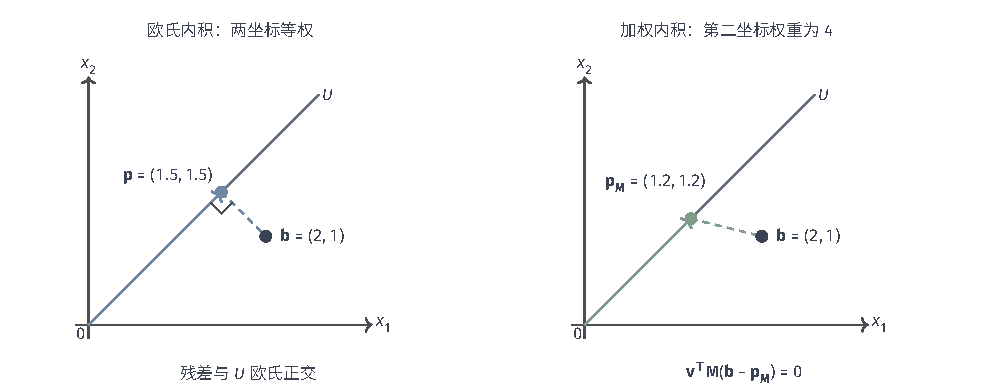
\includegraphics[width=168.998mm]{figures/00-shared/mathematical-preliminaries-upper/02-linear-spaces/tikz/linear-algebra-weighted-projection/figure.pdf}
  \caption{同一目标在同一直线上的欧氏投影与加权投影。实箭头是投影向量，虚线是残差；
  右图画在普通坐标中，残差不必形成欧氏直角。正交性必须用所选内积判断。}
  \label{fig:linear-algebra-weighted-projection}
\end{figure*}



加权问题可以化回普通问题。由定理~\ref{thm:ls-gram-factor}，正定$\bm M$可写成
$\bm M=\bm R^\top\bm R$，$\bm R$可逆。于是
$(\bm A\bm x-\bm b)^\top\bm M(\bm A\bm x-\bm b)=\lVert\bm R\bm A\bm x-\bm R\bm b\rVert_2^2$。
令$\tilde{\bm A}=\bm R\bm A$、$\tilde{\bm b}=\bm R\bm b$，加权目标就是普通平方残差$\lVert\tilde{\bm A}\bm x-\tilde{\bm b}\rVert_2^2$，
加权正规方程~\eqref{eq:linear-algebra-weighted-normal-equations}就是$\tilde{\bm A}^\top\tilde{\bm A}\hat{\bm x}=\tilde{\bm A}^\top\tilde{\bm b}$。
这一步常称\term{白化}（whitening）：先用$\bm R$把各坐标的误差变换到同一欧氏尺度。
于是前面的结论都可以搬过来：加权正规方程总有解；$\bm R$可逆使$\ker\tilde{\bm A}=\ker\bm A$，
所以解唯一的条件仍是$\bm A$满列秩。权重只移动最近点，不改变唯一性。

计算时把$\bm A,\bm b,\bm M$作为输入，先用Cholesky得到权重因子$\bm R$，再形成$\tilde{\bm A},\tilde{\bm b}$。对这对数据运行前面的QR或迭代最小二乘求解器，所得$\hat{\bm x}$就是原变量的解，无需再次变换未知量。输出时核验$\bm A^\top\bm M(\bm b-\bm A\hat{\bm x})$，并报告加权残差长度；普通残差的欧氏正交性已经不是这里的最优性条件。

\subsection{结果检验}
\label{sec:ls-least-squares-verification}

最小二乘的残差一般不为零，所以“残差小”不能作为合格标准；合格标准是残差与列空间正交。
算出$\hat{\bm x}$后分别核验三项。第一，正规方程残差$\bm g=\bm A^\top(\bm b-\bm A\hat{\bm x})$是否在容限内为零，
它检验的正是正交性判据。第二，输出残差$\bm r=\bm b-\bm A\hat{\bm x}$的长度，它是$\bm b$到列空间的距离，
说明模型能解释观测到什么程度。第三，若要求最小范数解，检查$\hat{\bm x}$是否与$\ker\bm A$正交。

用示例~\ref{ex:ls-normal-equations-three-by-two}核对：$\hat{\bm x}=(1,2)^\top$时$\bm r=(1,1,-1)^\top$，$\bm A^\top\bm r=(0,0)^\top$，第一项通过；
$\lVert\bm r\rVert_2=\sqrt3$，这是无法再减小的距离；$\bm A$满列秩，$\ker\bm A=\{\bm0\}$，第三项自动满足。

加权问题按原目标核验：检查加权正规方程~\eqref{eq:linear-algebra-weighted-normal-equations}的残差
$\bm A^\top\bm M(\bm b-\bm A\hat{\bm x})$，并报告$\bm M$加权的残差长度。白化后的残差（用$\bm M=\bm R^\top\bm R$的因子$\bm R$变换后的$\bm R\bm r$）与它长度相同，
但坐标已经变换，不能当作原观测的残差逐项解读。

\section{线性方程与最小二乘方法的比较}

前面的算法都围绕线性关系展开，但返回的对象并不相同。选择方法前，应先确定任务要求满足方程、最小化残差，还是在多个最优解中选出长度最小的一个；随后再检查矩阵结构和可用的数据访问方式。

\subsection{求解目标与方法适用性}

相容方程要求原残差为零。若零空间非平凡，这仍不能唯一决定未知量：从一个解加上任何零空间向量，输出都不变。最小范数要求解与零空间正交，是额外的选解条件。

不相容问题的原残差不能消失。欧氏最小二乘要求正规残差为零；如果又要求最小范数，还须使解位于行空间。因而“残差下降”“达到最小二乘解”和“得到最小范数解”是三种不同的判断，不能用同一个停止量代替。

\subsection{矩阵条件}

表中“矩阵作用”指能够计算矩阵与向量的乘积，不必保存整个矩阵。迭代法的条件指本章已经建立保证的情形；一般矩阵上的表现不能由方法名称保证。

\begin{center}
\small
\begin{tabular}{p{0.24\textwidth}p{0.65\textwidth}}
\toprule
方法 & 适用条件与主要输出\\
\midrule
LU & 可逆方阵；选主元消元后求精确方程的解\\
Cholesky & 对称正定方阵；分解可供多个右端复用\\
块LDL$^\top$ & 对称可逆矩阵，可含不定性；需要对称选主元\\
Schur补 & 已知分块且被消去的块可逆；先求约化方程\\
Woodbury & 已有可复用的基矩阵求解器，更新秩较低\\
Richardson & 对称正定时可按谱范围选步长；只用矩阵作用\\
Jacobi & 对角非零；严格行对角占优保证收敛，正定本身不够\\
Gauss--Seidel & 严格行对角占优或对称正定；逐行原位更新\\
SOR、SSOR & 对称正定且$0<\omega<2$；顺序扫掠或双向扫掠\\
CG & 对称正定；短递推，最小化能量范数误差\\
GMRES & 一般非奇异方阵；最小化原残差，需保存搜索基\\
MINRES & 对称非奇异方阵，可不定；最小化原残差\\
BiCG & 一般非对称方阵；需要矩阵及转置作用，可能失效\\
BiCGSTAB & 一般非对称方阵；无需转置作用，仍须检查失效\\
\bottomrule
\end{tabular}
\end{center}

矩形问题还需要比较求解目标。下面几种方法直接以最小二乘或行投影为出发点，不必先把原矩阵改成方阵。

\begin{center}
\small
\begin{tabular}{p{0.24\textwidth}p{0.65\textwidth}}
\toprule
方法 & 适用条件与主要输出\\
\midrule
正规方程法 & 满列秩最小二乘；形成正规矩阵会平方条件数\\
QR & 满列秩最小二乘；正交变换后求三角方程\\
SVD & 包括秩亏情形；给出秩、最小残差与最小范数代表\\
LSQR、LSMR & 矩形矩阵与转置作用；分别侧重原残差和正规残差\\
Kaczmarz & 相容系统，逐行访问；零初值选出最小范数解\\
扩展Kaczmarz & 允许不相容，需行列访问及辅助向量；概率保证另论\\
\bottomrule
\end{tabular}
\end{center}

左乘可逆矩阵保持精确方程的解集，却一般改变不相容问题中残差的权重。右换元保持可达到的输出，但欧氏最小范数随坐标尺度改变。把问题转换成某算法能够接收的形状以后，还要检查求解目标是否仍是原来的目标。

\subsection{计算开销与收敛速度}

稠密$n$阶LU、Cholesky、QR分解的工作量都为$O(n^3)$，因子的存储为$O(n^2)$；Cholesky利用对称性减少常数。分解完成后，每个新右端通常只需$O(n^2)$的三角求解。对$m\ge d$的稠密矩形矩阵，QR的主要工作量为$O(md^2)$。稀疏情形不能直接把这些估计中的维数换成非零元数，因为消元可能产生填充。

若矩阵有$s$个非零元，一次矩阵作用通常为$O(s)$。CG与BiCGSTAB等短递推保存常数个工作向量；完整GMRES的第$k$步还需对$k$个旧向量正交化，增加$O(kn)$工作和$O(kn)$存储。LSQR与LSMR每步使用一次矩阵作用和一次转置作用，工作向量总长度与$m+d$同阶。重正交化会改变这一存储估计。

因此总成本是每轮代价乘以达到要求所需的轮数，还要加上预条件构造和应用成本。只比较迭代次数，或只比较一次矩阵作用，都不足以判断哪个方法更省。

\subsection{数值稳定性}

正交变换避免了换基中的长度放大，因而QR常比显式形成正规方程更可靠；它仍不能消除原矩阵的小奇异值。SVD揭示这些方向，却也不能从带噪数据中恢复本来就不确定的分量。截断和惩罚会改变问题，应与单纯改善计算过程区别开来。

迭代结束时重新计算原残差。最小二乘还检查正规残差，并结合矩阵尺度解释容差。递推残差很小而真实残差较大，说明舍入误差已影响递推；相邻解几乎不变则可能只是停滞。若数据本身只精确到一定尺度，过度降低计算残差未必改善最终解。

\subsection{典型场景中的取舍}

对中等规模的稠密可逆方阵，可以从带选主元LU开始；若已知对称正定，改用Cholesky。多个右端共用矩阵时，复用分解通常比重复启动迭代更合适。已有分解而矩阵只发生低秩修改时，再检查Woodbury的小系统是否可逆、是否值得复用。

对大型稀疏对称正定系统，可以使用预条件CG；对称不定时考虑保持对称结构的MINRES。一般非对称系统中，GMRES用较多存储换取明确的残差最小化，BiCGSTAB用短递推减少存储，但需接受残差波动及失效检查。

对稠密矩形最小二乘，满列秩时可用QR；需要识别秩或最小范数时使用SVD。大型矩形问题若提供矩阵与转置作用，可用LSQR或LSMR；只方便逐行读取且系统相容时，行投影才直接符合数据访问方式。算法的选择由目标、结构与成本共同决定。


\section{伪逆}
\label{sec:ls-pseudoinverse}

到这里，三种情况各有各的答案。$\bm A$可逆时，唯一解是$\bm A^{-1}\bm b$；满行秩而有无穷多解时，
最小范数解是$\bm A^\top(\bm A\bm A^\top)^{-1}\bm b$；满列秩而无解时，最小二乘解是$(\bm A^\top\bm A)^{-1}\bm A^\top\bm b$。
三个公式各自要求一种满秩，而一般的$\bm A$可能既不满行秩、也不满列秩，这时方程可能无解，
最小二乘解又不唯一，需要先取最近点、再在最近点的全部原像中取范数最小者。
本小节用第~\ref{chap:linear-analysis}章的奇异值分解构造一个矩阵$\bm A^\dagger$，
使$\bm A^\dagger\bm b$在任何秩下都给出这样两次选择的结果，再说明前面三个公式都是它的特例。

\subsection{用SVD构造统一的解}

设$\bm A\in\mathbb R^{m\times d}$的秩为$r$，奇异值分解为~\eqref{eq:matrix-analysis-svd-rank-one-sum}，
$\sigma_1\geq\cdots\geq\sigma_r>0$；按第~\ref{sec:ls-svd}节的构造，把$\bm u_1,\ldots,\bm u_r$与$\bm v_1,\ldots,\bm v_r$
分别扩充为$\mathbb R^m$与$\mathbb R^d$的标准正交基。那里已经说明，$\operatorname{range}(\bm A)$由$\bm u_1,\ldots,\bm u_r$张成，
$\ker\bm A$由$\bm v_{r+1},\ldots,\bm v_d$张成。

$\bm A$把$\bm v_i$伸缩为$\sigma_i\bm u_i$，反向自然应把$\bm u_i$送回$\bm v_i/\sigma_i$。
按两次选择的要求分配$\bm b$的各个分量：把$\bm b$按$\bm u_i$展开，分量$\bm u_i^\top\bm b$（$i\leq r$）配给$\bm v_i/\sigma_i$；
落在$\operatorname{range}(\bm A)^\perp$中的分量（$i>r$）没有原像，直接丢弃，这对应取最近点；
零空间方向$\bm v_{r+1},\ldots,\bm v_d$不分配任何分量，这对应在原像中取范数最小者。

\begin{definition}[Moore--Penrose伪逆]
\label{def:matrix-analysis-pseudoinverse}
设$\bm A$有奇异值分解~\eqref{eq:matrix-analysis-svd-rank-one-sum}。$\bm A$的\term{Moore--Penrose伪逆}（Moore--Penrose pseudoinverse）为
\begin{equation}
 \bm A^\dagger=\sum_{i=1}^r\frac{1}{\sigma_i}\bm v_i\bm u_i^\top,
 \label{eq:matrix-analysis-pseudoinverse}
\end{equation}
$\bm A=\bm0$时规定$\bm A^\dagger=\bm0$。
\end{definition}

用于计算时不必先形成整个伪逆矩阵。输入$\bm A,\bm b$后，计算紧致SVD；对每个非零奇异值依次计算$c_i=\bm u_i^\top\bm b$与$z_i=c_i/\sigma_i$，最后组合$\hat{\bm x}=\sum_{i=1}^r z_i\bm v_i$。输出包含解及原残差；若数据只能确定数值秩，还要报告采用的阈值，因为丢掉正的小奇异值就转为后面的截断求解。

下面在精确秩已知的条件下，证明这样构造的矩阵恰好完成了上面的两次选择。
\begin{theorem}[最小二乘与最小范数]
\label{thm:matrix-analysis-pseudoinverse-minimum-norm}
给定$\bm A\in\mathbb R^{m\times d}$和$\bm b\in\mathbb R^m$，全部最小二乘解为
\begin{equation}
\begin{gathered}
\hat{\bm x}=\bm A^\dagger\bm b+\bm z\\
\bm z\in\ker\bm A,
\end{gathered}
\label{eq:ls-all-pseudoinverse-solutions}
\end{equation}
其中$\bm A^\dagger\bm b$是唯一的最小欧氏范数解；方程相容时，它就是全部精确解中范数最小者。
\end{theorem}
\begin{proof}
把$\bm b$与$\bm x$分别按左、右奇异向量展开，记$b_i=\bm u_i^\top\bm b$、$c_i=\bm v_i^\top\bm x$。由$\bm A\bm x=\sum_{i\leq r}\sigma_ic_i\bm u_i$与$\bm u_1,\ldots,\bm u_m$标准正交，
\[
 \lVert\bm A\bm x-\bm b\rVert_2^2
 =\sum_{i=1}^r(\sigma_ic_i-b_i)^2+\sum_{i=r+1}^m b_i^2 .
\]
第二项与$\bm x$无关；第一项当且仅当$c_i=b_i/\sigma_i$（$i\leq r$）时为零，而$c_{r+1},\ldots,c_d$可以任取。前者正是$\bm A^\dagger\bm b$的坐标，后者组成$\ker\bm A$中的任意向量，所以最小二乘解恰为$\bm A^\dagger\bm b+\bm z$，$\bm z\in\ker\bm A$。由于$\bm A^\dagger\bm b$只含$\bm v_1,\ldots,\bm v_r$方向，它与$\bm z$正交，$\lVert\bm x\rVert_2^2=\lVert\bm A^\dagger\bm b\rVert_2^2+\lVert\bm z\rVert_2^2$，最小值仅在$\bm z=\bm0$时达到。方程相容时第二项为零，最小二乘解就是精确解，论证不变。
\end{proof}

\paragraph{三种情况的统一}

定理对$\bm A$的秩和$\bm b$的位置都没有要求，所以前面分别处理的情况都包含在其中。
方程相容时，最近点就是$\bm b$本身，$\bm A^\dagger\bm b$是精确解中范数最小的一个：解唯一时它就是那个解，
有无穷多解时它就是第~\ref{sec:ls-select-among-solutions}节的最小范数解。方程无解时，$\bm A^\dagger\bm b$是最小二乘解；
最小二乘解唯一时它就是那一个，不唯一时它是其中范数最小者。

三个满秩公式由此成为特例。$\bm A$满列秩时$\ker\bm A=\{\bm0\}$，最小二乘解唯一，
所以对每个$\bm b$都有$\bm A^\dagger\bm b=(\bm A^\top\bm A)^{-1}\bm A^\top\bm b$，即$\bm A^\dagger=(\bm A^\top\bm A)^{-1}\bm A^\top$。
$\bm A$满行秩时每个右端都相容，$\bm A^\dagger\bm b$是最小范数精确解，由第~\ref{sec:ls-select-among-solutions}节，
$\bm A^\dagger=\bm A^\top(\bm A\bm A^\top)^{-1}$。$\bm A$可逆时两种情形同时成立，两个公式都化为$\bm A^{-1}$，所以$\bm A^\dagger=\bm A^{-1}$。
下面用一个欠定方程核对满行秩的情形。

\begin{example}[欠定方程的伪逆]
\label{ex:ls-pinv-underdetermined}
欠定方程$2x_1=3$的系数矩阵$\bm A=[2\ 0]$满行秩，右端$\bm b=(3)$。$\bm A$的奇异值分解只有一项：
$\sigma_1=2$、$\bm u_1=(1)$、$\bm v_1=(1,0)^\top$。和式~\eqref{eq:matrix-analysis-pseudoinverse}给出
\[
 \bm A^\dagger=\frac12\bm v_1\bm u_1^\top=\begin{bmatrix}1/2\\0\end{bmatrix},
\]
与满行秩公式$\bm A^\top(\bm A\bm A^\top)^{-1}=(2,0)^\top/4$一致。$\bm A^\dagger\bm b=(3/2,0)^\top$
正是全部解$(3/2,t)^\top$中范数最小的一个。
\end{example}

秩亏而又不相容时，两次选择都真正起作用，满秩公式一个也用不上。

\begin{example}[秩亏且不相容时的两次选择]
\label{ex:ls-pinv-two-selections}
取$\bm A=\left[\begin{smallmatrix}1&1\\0&0\end{smallmatrix}\right]$、$\bm b=(2,1)^\top$。$\bm A$的秩为$1$，既不满行秩，也不满列秩。
可达输出都形如$(s,0)^\top$，其中离$\bm b$最近的是$(2,0)^\top$，残差$(0,1)^\top$无法消除。
$(2,0)^\top$的原像是直线$x_1+x_2=2$，由示例~\ref{ex:ls-min-norm-line}，其上最靠近原点的点是$(1,1)^\top$。
用和式核对：$\bm A$只有一个正奇异值$\sigma_1=\sqrt2$，对应$\bm u_1=(1,0)^\top$、$\bm v_1=(1,1)^\top/\sqrt2$，于是
\[
\begin{gathered}
\bm A^\dagger=\frac1{\sqrt2}\bm v_1\bm u_1^\top=\frac12\begin{bmatrix}1&0\\1&0\end{bmatrix}\\
\bm A^\dagger\bm b=\begin{bmatrix}1\\1\end{bmatrix}.
\end{gathered}
\]
两次选择的结果与和式一致。
\end{example}

图~\ref{fig:matrix-analysis-pseudoinverse-selections}画出这两次选择。
伪逆既没有让无解的方程变得可解，也没有恢复被$\bm A$消去的信息，它只是在两处都作了最小化选择。

\begin{figure*}[htbp]
  \centering
  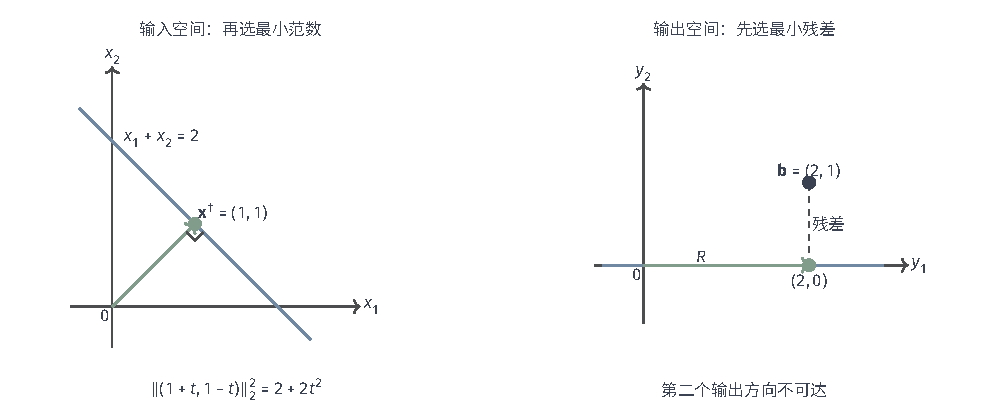
\includegraphics[width=168.998mm]{figures/00-shared/mathematical-preliminaries-upper/02-linear-spaces/tikz/matrix-analysis-pseudoinverse-selections/figure.pdf}
  \caption{伪逆的两次选择。右图先在可达输出中选择离$\bm b=(2,1)^\top$最近的
  $(2,0)^\top$；左图再在整条原像直线$x_1+x_2=2$上选择最靠近原点的$(1,1)^\top$。
  两图属于不同空间，各自等比例绘制。}
  \label{fig:matrix-analysis-pseudoinverse-selections}
\end{figure*}

\subsection{Penrose条件与两个投影}

两次选择也可以用投影矩阵表达。由和式直接相乘，
\[
 \begin{gathered}
\bm A\bm A^\dagger=\sum_{i\leq r}\bm u_i\bm u_i^\top\\
\bm A^\dagger\bm A=\sum_{i\leq r}\bm v_i\bm v_i^\top ,
 \end{gathered}
\]
前者是到$\operatorname{range}(\bm A)$的正交投影，后者是到$(\ker\bm A)^\perp=\operatorname{range}(\bm A^\top)$的正交投影
（式~\eqref{eq:linear-algebra-orthogonal-projector}）。也就是说，$\bm A^\dagger$先把输出正交投影到$\operatorname{range}(\bm A)$，
再在$\operatorname{range}(\bm A^\top)$上反演$\bm A$。

奇异值分解并不唯一，伪逆却不依赖分解的具体选取。由上面两个投影，$\bm A^\dagger$满足四条Penrose条件：
\[
 \begin{gathered}
\bm A\bm A^\dagger\bm A=\bm A\\
\bm A^\dagger\bm A\bm A^\dagger=\bm A^\dagger\\
(\bm A\bm A^\dagger)^\top=\bm A\bm A^\dagger\\
(\bm A^\dagger\bm A)^\top=\bm A^\dagger\bm A .
 \end{gathered}
\]
满足这四条的矩阵只有一个，所以无论用哪个奇异值分解代入和式，得到的都是同一个矩阵。

下面证明唯一性。

设$\bm G$也满足四条条件。由第一条，$(\bm A\bm G)^2=(\bm A\bm G\bm A)\bm G=\bm A\bm G$，即$\bm A\bm G$幂等，
且$\operatorname{range}(\bm A\bm G)=\operatorname{range}(\bm A)$（$\subseteq$显然，$\supseteq$由$\bm A=\bm A\bm G\bm A$）；
同理$\bm G\bm A$幂等，且$\ker(\bm G\bm A)=\ker\bm A$（$\supseteq$显然，$\subseteq$由$\bm A=\bm A\bm G\bm A$）。
后两条说明它们对称，而由第~\ref{sec:ls-projection-matrices}节，对称的幂等矩阵就是到其像的正交投影。
$\bm A\bm G$与$\bm A\bm A^\dagger$都是到$\operatorname{range}(\bm A)$的正交投影，所以$\bm A\bm G=\bm A\bm A^\dagger$。
对称矩阵的像是其零空间的正交补，所以$\bm G\bm A$与$\bm A^\dagger\bm A$都是到$(\ker\bm A)^\perp$的正交投影，$\bm G\bm A=\bm A^\dagger\bm A$。再由第二条，
\[
 \bm G=\bm G\bm A\bm G=(\bm A^\dagger\bm A)\bm G=\bm A^\dagger(\bm A\bm G)=\bm A^\dagger\bm A\bm A^\dagger=\bm A^\dagger .
\]

至此，三种情况的答案统一为$\bm A^\dagger\bm b$。实际计算中，满秩时仍用前面各小节基于分解的方法，
不必为此计算奇异值分解；伪逆的作用在于给出一个对任何秩都成立的统一描述。

不过伪逆有一个与逆矩阵不同的性质：它关于矩阵不连续。非零标量$\varepsilon$的伪逆是$1/\varepsilon$，零的伪逆却是$0$，
$\varepsilon\to0$时前者趋于无穷，而不是趋于后者。原因在于和式中的增益$1/\sigma_i$：小奇异值被放大成大增益。
数据带有误差时，这种放大意味着什么，是下一节要回答的问题。

\section{方程与最小二乘的误差分析}
\label{sec:ls-numerical-sensitivity}

前面各小节都假定$\bm A$与$\bm b$精确，并在精确算术下求解。实际数据带有测量误差，计算又有舍入误差，
所以还要问：输入有一点误差时，算出的解会偏离多少？残差小时，解是否就准确？
第~\ref{chap:linear-analysis}章已经回答了最简单的情形：可逆方程只有右端带误差时，
解的相对误差不超过条件数$\kappa(\bm A)$乘右端的相对误差（定理~\ref{thm:matrix-analysis-condition-number-bound}），
而在欧氏范数下$\kappa_2(\bm A)$是最大与最小奇异值之比。本节从这里出发，先处理系数矩阵也带误差的情形，
再说明真解未知时怎样由残差判断算出的解，然后分析最小二乘的三类输出。分析会显示，误差放大的根源都在小奇异值，
求解方法还可能额外放大误差；最后据此介绍数据与计算两方面的改进。

\subsection{右端项与系数矩阵的有限扰动}
\label{sec:ls-equation-sensitivity}
\label{sec:ls-linear-system-sensitivity}

\paragraph{右端扰动}

先看只改右端的情形。

设$\bm A$可逆，右端由$\bm b$变为$\bm b+\Delta\bm b$，解的变化为$\Delta\bm x=\bm A^{-1}\Delta\bm b$。
由$\lVert\bm A^{-1}\rVert_2=1/\sigma_{\min}(\bm A)$，右端误差落在小奇异值方向时被放大$1/\sigma_{\min}$倍；
换成相对误差，放大倍数不超过$\kappa(\bm A)$。下面用两个$2\times2$例子对照。

\begin{example}[良态方程的右端扰动]
\label{ex:ls-rhs-perturbation-well-conditioned}
取$\bm A_1=\operatorname{diag}(2,1)$，$\kappa_2(\bm A_1)=2$。右端由$(2,1)^\top$改为$(2,1.01)^\top$，解由$(1,1)^\top$变为$(1,1.01)^\top$。
两者的相对变化分别为
\[
 \begin{gathered}
\frac{\lVert\Delta\bm b\rVert_2}{\lVert\bm b\rVert_2}=\frac{0.01}{\sqrt5}\approx0.00447\\
\frac{\lVert\Delta\bm x\rVert_2}{\lVert\bm x\rVert_2}=\frac{0.01}{\sqrt2}\approx0.00707,
 \end{gathered}
\]
放大约$1.58$倍，不超过$\kappa_2(\bm A_1)=2$。
\end{example}

\begin{example}[近平行列的右端扰动]
\label{ex:ls-rhs-perturbation-near-parallel}
取$\bm A_2=\left[\begin{smallmatrix}1&1\\0&\varepsilon\end{smallmatrix}\right]$，$0<\varepsilon\ll1$，两列接近同向。
$\bm A_2^\top\bm A_2=\left[\begin{smallmatrix}1&1\\1&1+\varepsilon^2\end{smallmatrix}\right]$的迹为$2+\varepsilon^2$、行列式为$\varepsilon^2$，
两个特征值约为$2$与$\varepsilon^2/2$，所以$\sigma_{\max}\approx\sqrt2$、$\sigma_{\min}\approx\varepsilon/\sqrt2$，$\kappa_2(\bm A_2)\approx2/\varepsilon$。

取$\varepsilon=10^{-2}$、$\bm b=(2,0)^\top$，解为$(2,0)^\top$。只把$\bm b$的第二分量改为$\eta=10^{-2}$，
由$\varepsilon x_2=\eta$与$x_1+x_2=2$得新解$(1,1)^\top$。两者的相对变化分别为
\[
 \begin{gathered}
\frac{\lVert\Delta\bm b\rVert_2}{\lVert\bm b\rVert_2}=\frac{\eta}{2}=0.005\\
\frac{\lVert\Delta\bm x\rVert_2}{\lVert\bm x\rVert_2}=\frac{\lVert(-1,1)^\top\rVert_2}{\lVert(2,0)^\top\rVert_2}=\frac{\sqrt2}{2}\approx0.707,
 \end{gathered}
\]
放大约$141$倍，与$\kappa_2(\bm A_2)\approx200$同量级。
\end{example}

两个例子都没有舍入误差，差别完全来自问题本身。第二例中解的变化$(-1,1)^\top$几乎正沿着$\bm A_2$的小奇异值方向，
所以被放大得最多。

\paragraph{逆矩阵的扰动}
\label{sec:ls-inverse-sensitivity}
\label{sec:ch06-inverse-stability}

$\bm A$本身也带误差时，扰动后的矩阵甚至可能不再可逆。所以设$\bm B=\bm A+\bm E$，要先回答两件事：
$\bm B$是否可逆，$\bm B^{-1}$离$\bm A^{-1}$多远。答案会给出一个“到奇异边界的余量”。

先看可逆性。若$\lVert\bm A^{-1}\bm E\rVert<1$，则$\bm B$可逆。假设$\bm B\bm x=\bm0$，即$\bm A\bm x=-\bm E\bm x$，左乘$\bm A^{-1}$得$\bm x=-\bm A^{-1}\bm E\bm x$，取范数得$\lVert\bm x\rVert\leq\lVert\bm A^{-1}\bm E\rVert\lVert\bm x\rVert$，这只在$\bm x=\bm0$时可能，所以$\ker\bm B=\{\bm0\}$。

再看逆的变化。由$\bm B^{-1}(\bm A-\bm B)\bm A^{-1}=\bm B^{-1}-\bm A^{-1}$，逆差满足精确恒等式
\begin{equation}
 \bm B^{-1}-\bm A^{-1}
 =-\bm B^{-1}\bm E\,\bm A^{-1}.
 \label{eq:ch06-inverse-finite-perturbation}
\end{equation}
右端含有未知的$\bm B^{-1}$，需要先估计它的大小。

对任意$\bm y$，令$\bm x=\bm B^{-1}\bm y$，由$\bm A\bm x=\bm y-\bm E\bm x$得$\bm x=\bm A^{-1}\bm y-\bm A^{-1}\bm E\bm x$，取范数并移项，$\lVert\bm x\rVert\leq\lVert\bm A^{-1}\rVert\lVert\bm y\rVert/(1-\lVert\bm A^{-1}\bm E\rVert)$，即
\[
 \lVert\bm B^{-1}\rVert\leq\frac{\lVert\bm A^{-1}\rVert}{1-\lVert\bm A^{-1}\bm E\rVert}.
\]
代入恒等式，$\lVert\bm B^{-1}-\bm A^{-1}\rVert\leq\lVert\bm B^{-1}\rVert\lVert\bm E\rVert\lVert\bm A^{-1}\rVert$。两边除以$\lVert\bm A^{-1}\rVert$，并用$\lVert\bm A^{-1}\bm E\rVert\leq\lVert\bm A^{-1}\rVert\lVert\bm E\rVert=\kappa(\bm A)\lVert\bm E\rVert/\lVert\bm A\rVert$。为了用这个较易计算的上界替换分母，还需假设$\kappa(\bm A)\lVert\bm E\rVert/\lVert\bm A\rVert<1$；在此条件下得到
\[
 \frac{\lVert\bm B^{-1}-\bm A^{-1}\rVert}
      {\lVert\bm A^{-1}\rVert}
 \leq
 \frac{\kappa(\bm A)\,\lVert\bm E\rVert/\lVert\bm A\rVert}
      {1-\kappa(\bm A)\,\lVert\bm E\rVert/\lVert\bm A\rVert}.
\]
分子是条件数乘相对扰动，分母是到奇异边界的余量。$\kappa(\bm A)\lVert\bm E\rVert/\lVert\bm A\rVert$接近$1$时界急剧变大；
它不小于$1$时本界失效，但这不等于$\bm B$一定奇异。下面的对角例子说明，这个界可以取等号，余量趋于零时逆矩阵的变化确实无界。

\begin{example}[接近奇异边界的对角矩阵]
\label{ex:ls-inverse-perturbation-diagonal}
取$\bm A=\operatorname{diag}(1,\varepsilon)$，$0<\varepsilon<1$，则$\kappa_2(\bm A)=1/\varepsilon$。
令$\bm E=\operatorname{diag}(0,-\delta)$，$0<\delta<\varepsilon$，即把第二个对角元减少$\delta$。
逆矩阵的该元由$1/\varepsilon$变为$1/(\varepsilon-\delta)$，相对变化为
\[
 \frac{\lVert\bm B^{-1}-\bm A^{-1}\rVert_2}{\lVert\bm A^{-1}\rVert_2}
 =\frac{1/(\varepsilon-\delta)-1/\varepsilon}{1/\varepsilon}
 =\frac{\delta}{\varepsilon-\delta}.
\]
扰动的相对大小为$\lVert\bm E\rVert_2/\lVert\bm A\rVert_2=\delta$，于是$\kappa_2(\bm A)\lVert\bm E\rVert_2/\lVert\bm A\rVert_2=\delta/\varepsilon$，
上界为$(\delta/\varepsilon)/(1-\delta/\varepsilon)=\delta/(\varepsilon-\delta)$，与实际变化恰好相等。
$\delta\to\varepsilon$时相对变化无界：扰动的相对大小接近$1/\kappa_2(\bm A)=\varepsilon$时，矩阵到达奇异边界。
\end{example}

\paragraph{矩阵与右端同时扰动}

有了逆矩阵的估计，就可以处理一般情形。

设$\bm A$可逆且$\bm b\ne\bm0$，原解$\bm x$因而非零。扰动后的方程为$(\bm A+\bm E)(\bm x+\Delta\bm x)=\bm b+\Delta\bm b$，减去$\bm A\bm x=\bm b$，得$\bm A\Delta\bm x=\Delta\bm b-\bm E\bm x-\bm E\Delta\bm x$。左乘$\bm A^{-1}$并取范数，
\[
 \lVert\Delta\bm x\rVert\leq\lVert\bm A^{-1}\rVert\bigl(\lVert\Delta\bm b\rVert+\lVert\bm E\rVert\lVert\bm x\rVert+\lVert\bm E\rVert\lVert\Delta\bm x\rVert\bigr).
\]
把含$\lVert\Delta\bm x\rVert$的项移到左边，两边除以$\lVert\bm x\rVert$，并用$\lVert\Delta\bm b\rVert/\lVert\bm x\rVert\leq\lVert\bm A\rVert\lVert\Delta\bm b\rVert/\lVert\bm b\rVert$，在$\kappa(\bm A)\lVert\bm E\rVert/\lVert\bm A\rVert<1$时得到
\begin{equation}
 \frac{\lVert\Delta\bm x\rVert}{\lVert\bm x\rVert}
 \leq
 \frac{\kappa(\bm A)}{1-\kappa(\bm A)\lVert\bm E\rVert/\lVert\bm A\rVert}
 \left(
 \frac{\lVert\Delta\bm b\rVert}{\lVert\bm b\rVert}
 +\frac{\lVert\bm E\rVert}{\lVert\bm A\rVert}
 \right).
 \label{eq:matrix-analysis-linear-system-perturbation}
\end{equation}
读法是：两类相对扰动先相加，再被条件数放大，最后除以到奇异边界的余量。
$\bm E=\bm0$时它退回定理~\ref{thm:matrix-analysis-condition-number-bound}的右端扰动界。
这仍是最坏方向上的上界；扰动是否落在放大方向，决定实际误差离这个上界有多远。

\subsection{残差、前向误差与后向误差}
\label{sec:ls-numerical-stability}
\label{sec:ls-data-computation-error}
\label{sec:linear-algebra-error-propagation}
\label{sec:ch06-error-propagation}
\label{sec:ls-result-verification}
\label{sec:matrix-analysis-error-verification}

上面的界比较的是两个精确解。实际手里只有一个算出的候选解$\widehat{\bm x}$，真解未知，怎样判断它的误差？以下仍设$\bm A$可逆且$\bm b\ne\bm0$。
第~\ref{sec:ls-linear-equation-verification}节用残差核验候选解，并提醒残差小不等于解准确；现在可以定量说明这一点。能直接计算的是残差
\begin{equation}
 \bm r=\bm b-\bm A\widehat{\bm x}.
 \label{eq:matrix-analysis-residual}
\end{equation}
由$\bm A(\bm x-\widehat{\bm x})=\bm r$，候选解的误差是$\bm A^{-1}\bm r$，与只改右端的情形相同，相对误差满足
\[
 \frac{\lVert\widehat{\bm x}-\bm x\rVert}{\lVert\bm x\rVert}
 \leq\kappa(\bm A)\frac{\lVert\bm r\rVert}{\lVert\bm b\rVert}.
\]
所以病态时小残差不保证解准确，下面的例子把这一点推到极端。

\begin{example}[反例：残差小而解误差大]
\label{ex:ls-small-residual-large-error}
取$\bm A=\operatorname{diag}(1,\varepsilon)$、$\bm b=(1,\varepsilon)^\top$，$0<\varepsilon\ll1$，精确解为$\bm x=(1,1)^\top$。
候选解$\widehat{\bm x}=(1,0)^\top$的残差为$\bm r=(0,\varepsilon)^\top$，相对残差为$\varepsilon/\sqrt{1+\varepsilon^2}$，随$\varepsilon\to0$趋于零；
相对解误差却是$\lVert(0,-1)^\top\rVert_2/\lVert(1,1)^\top\rVert_2=1/\sqrt2$，不随$\varepsilon$减小。
这与上面的界一致：$\kappa_2(\bm A)=1/\varepsilon$恰好抵消了相对残差中的因子$\varepsilon$。
\end{example}

残差还有另一种读法：把$\widehat{\bm x}$看作某个邻近问题的精确解，问这个邻近问题离原问题多近。
满足$(\bm A+\Delta\bm A)\widehat{\bm x}=\bm b+\Delta\bm b$的最小相对扰动称为\term{后向误差}（backward error）；
与之相对，直接比较答案的误差$\widehat{\bm x}-\bm x$称为\term{前向误差}（forward error）。
允许矩阵与右端同时改变、以相对大小$\max\{\lVert\Delta\bm A\rVert_2/\lVert\bm A\rVert_2,\lVert\Delta\bm b\rVert_2/\lVert\bm b\rVert_2\}$度量时，后向误差为
\begin{equation}
 \eta_2(\widehat{\bm x})
 =\frac{\lVert\bm r\rVert_2}
       {\lVert\bm A\rVert_2\lVert\widehat{\bm x}\rVert_2+\lVert\bm b\rVert_2}.
 \label{def:matrix-analysis-normwise-backward-error}
\end{equation}
先说明它不能更小：若$(\bm A+\Delta\bm A)\widehat{\bm x}=\bm b+\Delta\bm b$且两项相对大小都不超过$\epsilon$，则$\bm r=\Delta\bm A\widehat{\bm x}-\Delta\bm b$，
$\lVert\bm r\rVert_2\leq\epsilon(\lVert\bm A\rVert_2\lVert\widehat{\bm x}\rVert_2+\lVert\bm b\rVert_2)$，即$\epsilon\geq\eta_2$。
再说明它能达到。若$\widehat{\bm x}=\bm0$，取$\Delta\bm A=\bm0$、$\Delta\bm b=-\bm b$即可达到$\eta_2=1$。

若$\widehat{\bm x}\ne\bm0$，记分母为$d_0$，取
\[
 \begin{gathered}
\Delta\bm A=\frac{\lVert\bm A\rVert_2}{d_0\lVert\widehat{\bm x}\rVert_2}\,\bm r\widehat{\bm x}^\top\\
\Delta\bm b=-\frac{\lVert\bm b\rVert_2}{d_0}\,\bm r ,
 \end{gathered}
\]
则$(\bm A+\Delta\bm A)\widehat{\bm x}=\bm b-\bm r+\tfrac{\lVert\bm A\rVert_2\lVert\widehat{\bm x}\rVert_2}{d_0}\bm r=\bm b+\Delta\bm b$，两项的相对大小都等于$\eta_2$。

把后向误差当作式~\eqref{eq:matrix-analysis-linear-system-perturbation}中的数据扰动，就得到常用的经验规则：
前向误差大约不超过条件数乘后向误差。

后向误差的用处在于把算法的质量与问题的病态分开。计算机中的实数运算都有舍入，每次基本运算满足
\begin{equation}
\begin{gathered}
\operatorname{fl}(x\circ y)=(x\circ y)(1+\delta)\\
|\delta|\leq u,
\end{gathered}
\label{eq:ch06-floating-point-model}
\end{equation}
其中$\circ$是加减乘除之一，$u$称为单位舍入，双精度时$u=2^{-53}\approx1.1\times10^{-16}$。这个模型假设运算有定义且结果没有发生溢出或影响相对误差界的下溢。好的算法应当让这些舍入合起来只相当于一个很小的输入扰动。

\begin{definition}[后向稳定]
\label{def:matrix-analysis-backward-stability}
若算法对所有合法输入给出的结果都是某个邻近输入的精确解，且后向误差以$u$乘一个与数据无关的温和常数为界，则称算法\term{后向稳定}（backward stable）。
\end{definition}
正定矩阵的Cholesky分解与Householder QR（第~\ref{sec:ls-orthogonalization-qr}节）具有后向稳定性。带部分主元的LU分解，其后向误差界还依赖消元中的元素增长；增长温和时通常稳定，但不能对所有矩阵保证这个因子都很小。

示例~\ref{ex:ls-partial-pivoting}中不选主元的消元可能产生很大的乘子，把舍入误差放大成很大的输入扰动。

后向稳定只保证$\widehat{\bm x}$是邻近问题的精确解；病态问题中，很小的后向误差经条件数放大，仍可能得到很大的前向误差。
稳定算法不能治愈问题本身的病态，所以报告结果时要同时给出残差或后向误差，以及条件数的估计。

\subsection{最小二乘的不同输出与正规方程的风险}
\label{sec:ls-ls-regularization-sensitivity}
\label{sec:ls-ordinary-ls-sensitivity}

最小二乘有三类输出：系数$\hat{\bm x}=\bm A^\dagger\bm b$、拟合值$\bm A\hat{\bm x}=\bm P_{\operatorname{range}\bm A}\bm b$与残差$\bm b-\bm A\hat{\bm x}$。
它们对扰动的反应不同。

设$\bm A$固定、右端改变$\Delta\bm b$。拟合值的增量是$\bm P_{\operatorname{range}\bm A}\Delta\bm b$，正交投影不放大长度；
残差增量是$(\bm I-\bm P_{\operatorname{range}\bm A})\Delta\bm b$，同样不被放大；系数的增量却是$\bm A^\dagger\Delta\bm b$，
由伪逆的和式，$\lVert\Delta\hat{\bm x}\rVert_2\leq\lVert\Delta\bm b\rVert_2/\sigma_r$，其中$\sigma_r$是最小正奇异值；若$\bm A=\bm0$，伪逆为零，系数的增量也为零。
所以“拟合得好”与“系数可靠”是两回事，不能用一个误差数概括。

\paragraph{近共线设计}

示例~\ref{ex:ls-nearly-collinear-design}显示，拟合可以很好而系数很大。下面用奇异值说明原因。

\begin{example}[近共线设计的奇异值]
\label{ex:ls-nearly-collinear-singular-values}
示例~\ref{ex:ls-nearly-collinear-design}中设计矩阵$\bm X_\varepsilon$的两列是$\bm c_1$与$\bm c_1+\varepsilon\bm q$，
其中$\bm c_1=(1,1,1)^\top$、$\bm q=(0,1,-1)^\top$互相正交，所以两列都位于$\operatorname{span}\{\bm c_1,\bm q\}$内。
以$\bm c_1/\sqrt3$、$\bm q/\sqrt2$为这个平面的正交坐标，两列的坐标分别是$(\sqrt3,0)^\top$与$(\sqrt3,\sqrt2\,\varepsilon)^\top$；
再把全部输出统一除以$\sqrt3$，设计矩阵化为
\begin{equation}
\begin{gathered}
\bm X_{\widetilde\varepsilon}
 =\begin{bmatrix}1&1\\0&\widetilde\varepsilon\end{bmatrix}\\
\widetilde\varepsilon=\sqrt{2/3}\,\varepsilon .
\end{gathered}
\label{eq:matrix-analysis-nearly-collinear-design}
\end{equation}
换成正交坐标不改变奇异值，统一缩放只把奇异值同除以$\sqrt3$，不改变它们的比，所以条件数可以在$\bm X_{\widetilde\varepsilon}$上计算。

Gram矩阵$\bm X_{\widetilde\varepsilon}^\top\bm X_{\widetilde\varepsilon}=\left[\begin{smallmatrix}1&1\\1&1+\widetilde\varepsilon^2\end{smallmatrix}\right]$的迹为$2+\widetilde\varepsilon^2$，
行列式为$\widetilde\varepsilon^2$，特征值为
\begin{equation}
 \lambda_\pm
 =\frac{2+\widetilde\varepsilon^2
          \mathbin{\pm}\sqrt{4+\widetilde\varepsilon^4}}{2}.
 \label{eq:matrix-analysis-nearly-collinear-gram-eigenvalues}
\end{equation}
$\widetilde\varepsilon\to0$时$\lambda_+\to2$，$\lambda_-=\widetilde\varepsilon^2/\lambda_+\approx\widetilde\varepsilon^2/2$，
所以$\bm X_{\widetilde\varepsilon}$的奇异值$\sigma_{\max}\to\sqrt2$、$\sigma_{\min}\approx\widetilde\varepsilon/\sqrt2$，
条件数约为$2/\widetilde\varepsilon=\sqrt6/\varepsilon$。乘回$\sqrt3$，$\bm X_\varepsilon$本身的最小奇异值约为$\sqrt3\,\widetilde\varepsilon/\sqrt2=\varepsilon$。
\end{example}

大奇异值对应的方向近似为两个系数同增同减，小奇异值对应的方向近似为两个系数此增彼减。
响应在后一方向上的分量被放大约$1/\varepsilon$倍，这正是$\hat{\bm w}_\varepsilon$中$\delta/\varepsilon$项的来源。

化简后的$\bm X_{\widetilde\varepsilon}$与示例~\ref{ex:ls-rhs-perturbation-near-parallel}的近平行矩阵$\bm A_2$形状相同，
所以可以在$\bm A_2$上直接看到系数怎样分裂。

\begin{example}[近平行列的系数分裂]
\label{ex:ls-coefficient-splitting}
沿用示例~\ref{ex:ls-rhs-perturbation-near-parallel}的$\bm A_2=\left[\begin{smallmatrix}1&1\\0&\varepsilon\end{smallmatrix}\right]$，
把右端扰动写成一般的$\eta$。右端为$(2,0)^\top$时解为$(2,0)^\top$；右端变为$(2,\eta)^\top$时，由$\varepsilon x_2=\eta$与$x_1+x_2=2$得
\begin{equation}
\begin{gathered}
\hat{\bm x}=\begin{bmatrix}2-\eta/\varepsilon\\ \eta/\varepsilon\end{bmatrix}\\
\Delta\hat{\bm x}=\begin{bmatrix}-\eta/\varepsilon\\ \eta/\varepsilon\end{bmatrix}.
\end{gathered}
\label{eq:matrix-analysis-collinear-coefficient-perturbation}
\end{equation}
系数误差的长度$\sqrt2\,|\eta|/\varepsilon$是右端误差$|\eta|$的$\sqrt2/\varepsilon$倍，两个系数沿相反方向分开。
$\bm A_2$可逆，拟合值始终等于右端本身。
\end{example}

图~\ref{fig:matrix-analysis-coefficient-sensitivity}画出$\varepsilon$减小时两个系数怎样分开。

\begin{figure}
 \centering
 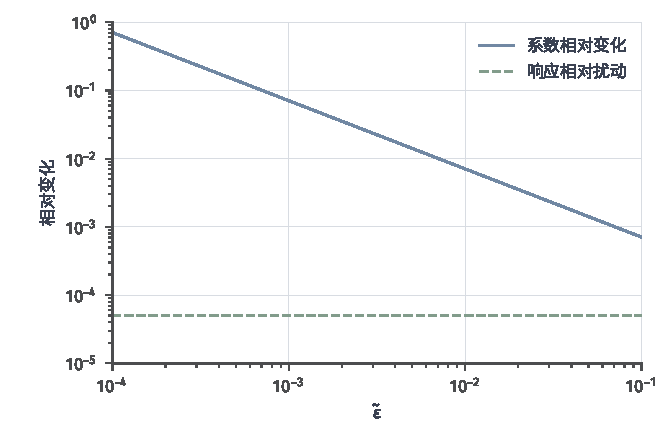
\includegraphics[width=0.92\linewidth]{figures/00-shared/mathematical-preliminaries-upper/02-linear-spaces/matplotlib/matrix-analysis-coefficient-sensitivity/figure.pdf}
 \caption{近平行列的系数分裂：对$\bm A_2=\left[\begin{smallmatrix}1&1\\0&\varepsilon\end{smallmatrix}\right]$固定右端扰动$\eta$，$\varepsilon$越小，两个系数
 沿相反方向偏离$(2,0)$越远，绝对误差随$1/\varepsilon$增长。}
 \label{fig:matrix-analysis-coefficient-sensitivity}
\end{figure}

\paragraph{正规方程的条件数平方}

问题本身的敏感度之外，求解方法也会影响结果。由奇异值分解，$\bm A^\top\bm A$的特征值是$\sigma_i^2$，故满列秩时
\begin{equation}
 \kappa_2(\bm A^\top\bm A)=\kappa_2(\bm A)^2.
 \label{eq:matrix-analysis-normal-equation-condition-square}
\end{equation}
平方的后果在近平行矩阵上看得最清楚。

\begin{example}[形成Gram矩阵时丢失的信息]
\label{ex:ls-gram-rounding-loss}
对示例~\ref{ex:ls-rhs-perturbation-near-parallel}的$\bm A_2$，$\kappa_2(\bm A_2)\approx2/\varepsilon$。
Gram矩阵$\bm A_2^\top\bm A_2=\left[\begin{smallmatrix}1&1\\1&1+\varepsilon^2\end{smallmatrix}\right]$的小特征值约为$\varepsilon^2/2$，条件数约为$4/\varepsilon^2$。
取$\varepsilon=10^{-8}$，则$\varepsilon^2=10^{-16}$已低于双精度的单位舍入$u\approx1.1\times10^{-16}$，
$1+\varepsilon^2$在舍入后就是$1$，存储下来的Gram矩阵成为奇异的$\left[\begin{smallmatrix}1&1\\1&1\end{smallmatrix}\right]$。
而$\bm A_2$本身的条件数约为$2\times10^8$，远未达到$1/u$，它的两列在双精度下仍可区分。
\end{example}

所以形成$\bm A^\top\bm A$这一步就可能把小奇异方向的信息丢掉。这就是第~\ref{sec:ls-qr-method}节的QR方法不形成$\bm A^\top\bm A$的原因：
用Householder反射实现时（第~\ref{sec:ls-orthogonalization-qr}节），它只经过正交变换，不会在问题本身的敏感度之外再把条件数平方。

\subsection{伪逆、秩变化与数值秩}

以上只改右端。矩阵本身改变时，秩是否保持起决定作用。设$\bm A$与$\bm B=\bm A+\bm E$的正奇异值都不小于$s_0>0$。
直接展开右端可验证恒等式
\[
 \bm B^\dagger-\bm A^\dagger
 =-\bm B^\dagger\bm E\bm A^\dagger
 +\bm B^\dagger(\bm I-\bm A\bm A^\dagger)
 -(\bm I-\bm B^\dagger\bm B)\bm A^\dagger .
\]
三项分别估计。非零矩阵满足$\lVert\bm A^\dagger\rVert_2=1/\sigma_r(\bm A)\leq1/s_0$；零矩阵的伪逆也是零，仍满足这个上界。对$\bm B$同理。
第一项不超过$\lVert\bm B^\dagger\rVert_2\lVert\bm E\rVert_2\lVert\bm A^\dagger\rVert_2\leq\lVert\bm E\rVert_2/s_0^2$。
第二项利用Penrose条件写$\bm B^\dagger=\bm B^\dagger(\bm B\bm B^\dagger)^\top=\bm B^\dagger(\bm B^\dagger)^\top\bm B^\top$；
又因$\bm A^\top(\bm I-\bm A\bm A^\dagger)=\bm0$，有$\bm B^\top(\bm I-\bm A\bm A^\dagger)=\bm E^\top(\bm I-\bm A\bm A^\dagger)$，
所以该项不超过$\lVert\bm B^\dagger\rVert_2^2\lVert\bm E\rVert_2\leq\lVert\bm E\rVert_2/s_0^2$。第三项同理。合起来，
\begin{equation}
 \lVert\bm B^\dagger-\bm A^\dagger\rVert_2
 \leq\frac{3\lVert\bm E\rVert_2}{s_0^2}.
 \label{eq:ch06-pseudoinverse-fixed-rank-perturbation}
\end{equation}
这个估计本身不要求两矩阵同秩，关键是它们的正奇异值有共同的正下界。若一列矩阵趋于$\bm A$而秩在极限处下降，就会有正奇异值趋于零，此时不能使用与扰动无关的$s_0$。相反，在固定秩且正奇异值远离零的邻域内，上界直接给出伪逆的连续性。

\begin{example}[反例：秩改变时伪逆不连续]
\label{ex:ls-pinv-discontinuity}
取$\bm A=\operatorname{diag}(1,0)$与$\bm B_\varepsilon=\operatorname{diag}(1,\varepsilon)$，$0<\varepsilon<1$。
二者之差$\lVert\bm B_\varepsilon-\bm A\rVert_2=\varepsilon\to0$，但
\[
 \begin{gathered}
\bm B_\varepsilon^\dagger=\operatorname{diag}(1,1/\varepsilon)\\
\bm A^\dagger=\operatorname{diag}(1,0),
 \end{gathered}
\]
所以$\lVert\bm B_\varepsilon^\dagger-\bm A^\dagger\rVert_2=1/\varepsilon\to\infty$。
$\bm B_\varepsilon$的秩为$2$，$\bm A$的秩为$1$；两者正奇异值的公共下界只能取$s_0=\varepsilon$，
界~\eqref{eq:ch06-pseudoinverse-fixed-rank-perturbation}给出$3\varepsilon/\varepsilon^2=3/\varepsilon$，同样随$\varepsilon\to0$无界。
\end{example}

这将伪逆一节末尾的标量现象扩展到了矩阵，也说明秩变化时新出现的小奇异值为何危险。

实际数据的秩因而要谨慎对待。第~\ref{chap:linear-analysis}章的奇异值扰动界~\eqref{eq:matrix-analysis-singular-value-perturbation}说明，矩阵改变$\bm E$时每个奇异值的移动不超过$\lVert\bm E\rVert_2$，所以小于数据误差尺度的奇异值与零无法区分：它可能是一个真实但很弱的方向，也可能只是噪声。据此，把大于某个阈值$\tau$的奇异值个数称为\term{数值秩}（numerical rank），$\tau$按数据误差的尺度选取。

综合本小节的分析：无论是方程的解、最小二乘的系数还是伪逆本身，误差放大都来自小奇异值。
它们一方面使增益$1/\sigma_i$很大，另一方面在误差尺度下难以与零区分；形成正规方程之类的计算步骤还会进一步损失精度。
前面的QR等方法避免额外引入不稳定计算；下一节转向正则化，通过改变目标来限制数据误差的放大。

\section{正则化与截断求解}
\label{sec:ls-truncated-svd-ridge}

小奇异值会把右端误差放大到解中。提高计算精度只能减少计算误差，不能消除数据本身的不确定性。本节通过限制小奇异值方向上的响应来换取稳定，同时明确所求的问题已发生改变。

\subsection{岭回归与Tikhonov正则化}
\label{sec:ls-regularized-ls}

示例~\ref{ex:ls-nearly-collinear-design}中，系数为了拟合上的微小改进而取得很大。若任务希望输入不要太大，
可以在数据项之外加上输入长度的平方惩罚，得到\term{岭回归}（ridge regression）
\begin{equation}
\begin{gathered}
\min_{\bm x}\ \lVert\bm A\bm x-\bm b\rVert_2^2+\lambda\lVert\bm x\rVert_2^2\\
\lambda>0.
\end{gathered}
\label{eq:ls-ridge-objective}
\end{equation}
参数$\lambda$权衡两项：$\lambda$越大，越倾向于小的输入，拟合误差不会减小；在某些退化情形下它也可能保持不变。

更一般地，惩罚可以作用在希望压小的量$\bm L\bm x$上，$\bm L\in\mathbb R^{p\times d}$，例如相邻分量之差，
得到\term{Tikhonov正则化}（Tikhonov regularization）\scite{math-hansen2008regtools}
\begin{equation}
\begin{gathered}
\min_{\bm x}\ \lVert\bm A\bm x-\bm b\rVert_2^2+\lambda\lVert\bm L\bm x\rVert_2^2\\
\lambda>0.
\end{gathered}
\label{eq:linear-algebra-general-tikhonov}
\end{equation}
两项都是平方长度，而$\lambda\lVert\bm L\bm x\rVert_2^2=\lVert\sqrt\lambda\,\bm L\bm x-\bm0\rVert_2^2$，
所以可以把两个残差向量上下堆成一个更长的残差向量，写成堆叠矩阵的普通最小二乘，
称为\term{增广最小二乘}（augmented least squares）：
\begin{equation}
 \begin{bmatrix}\bm A\\ \sqrt{\lambda}\,\bm L\end{bmatrix}\bm x
 \approx\begin{bmatrix}\bm b\\ \bm0\end{bmatrix}.
 \label{eq:ls-augmented-system}
\end{equation}
对堆叠矩阵套用正规方程~\eqref{eq:linear-algebra-normal-equations}：堆叠矩阵的转置乘自身是
$\bm A^\top\bm A+\lambda\bm L^\top\bm L$，转置乘堆叠右端是$\bm A^\top\bm b$，于是
\begin{equation}
 (\bm A^\top\bm A+\lambda\bm L^\top\bm L)\hat{\bm x}=\bm A^\top\bm b.
 \label{eq:ls-tikhonov-normal}
\end{equation}
它是普通最小二乘，存在性自动成立。由~\eqref{eq:ls-normal-kernel}，系数矩阵的零空间就是堆叠矩阵的零空间，
即同时满足$\bm A\bm x=\bm0$与$\bm L\bm x=\bm0$的向量，所以解唯一当且仅当
\begin{equation}
 \ker\bm A\cap\ker\bm L=\{\bm0\}.
 \label{eq:linear-algebra-tikhonov-common-nullspace}
\end{equation}
$\bm L=\bm I$时条件自动成立，岭回归对任意$\bm A$都有唯一解。其他惩罚则未必。

\begin{example}[反例：惩罚无法确定的方向]
\label{ex:ls-tikhonov-common-nullspace}
取$\bm A=\bm L=[\,1\ -1\,]$。两者的零空间都是$\operatorname{span}\{(1,1)^\top\}$，条件~\eqref{eq:linear-algebra-tikhonov-common-nullspace}不成立。
对任何解$\hat{\bm x}$和任何$t\in\mathbb R$，$\hat{\bm x}+t(1,1)^\top$的数据项与惩罚项都不变，因而也是解。
所以无论$\lambda$多大，都不能确定两个分量的共同水平。
\end{example}

权重与惩罚也可以同时使用，目标
$(\bm A\bm x-\bm b)^\top\bm M(\bm A\bm x-\bm b)+\lambda\lVert\bm L\bm x\rVert_2^2$的正规方程为
\begin{equation}
 (\bm A^\top\bm M\bm A+\lambda\bm L^\top\bm L)\hat{\bm x}=\bm A^\top\bm M\bm b,
 \label{eq:ls-general-normal-equations}
\end{equation}
$\bm M$正定、$\lambda>0$时，解唯一的条件仍是~\eqref{eq:linear-algebra-tikhonov-common-nullspace}。
要注意，加惩罚改变的是问题本身：选择$\lambda$是在重新设定任务，而不是让原方程“算得出来”的数值技巧。

$\lambda$怎样影响解，可以在奇异值坐标中读出。岭回归的正规方程是$(\bm A^\top\bm A+\lambda\bm I)\bm x=\bm A^\top\bm b$。在右奇异向量坐标$c_i=\bm v_i^\top\bm x$中，
$\bm A^\top\bm A$与$\bm I$同时成为对角矩阵，方程按方向分开：$i\leq r$时$(\sigma_i^2+\lambda)c_i=\sigma_i\,\bm u_i^\top\bm b$，
$i>r$时$\lambda c_i=0$，故$c_i=0$。于是
\begin{equation}
\begin{gathered}
\hat{\bm x}_\lambda=\sum_{i=1}^r\frac{\sigma_i}{\sigma_i^2+\lambda}\,(\bm u_i^\top\bm b)\,\bm v_i
 =\sum_{i=1}^r f_i\,\frac{\bm u_i^\top\bm b}{\sigma_i}\,\bm v_i\\
f_i=\frac{\sigma_i^2}{\sigma_i^2+\lambda}.
\end{gathered}
\label{eq:matrix-analysis-ridge-filter-factor}
\end{equation}
前一种写法说明，岭回归把伪逆中的增益$1/\sigma_i$换成了$\sigma_i/(\sigma_i^2+\lambda)$。由$\sigma_i^2+\lambda\geq2\sigma_i\sqrt\lambda$，
新的增益不超过$1/(2\sqrt\lambda)$，不再随$\sigma_i\to0$而爆炸。

后一种写法把它与最小范数解比较：每个方向多乘了一个介于$0$与$1$之间的\term{滤波因子}（filter factor）$f_i$。
$\sigma_i^2\gg\lambda$时$f_i\approx1$，该方向几乎不受影响；$\sigma_i^2\ll\lambda$时$f_i\approx\sigma_i^2/\lambda$，该方向被压低，增益约为$\sigma_i/\lambda$；
$\sigma_i^2=\lambda$处$f_i$恰为$1/2$。代价是大奇异值方向也被轻微压缩，$f_i$总小于$1$。下面在近共线设计上看两个$\lambda$的效果。

\begin{example}[近共线设计上的岭回归]
\label{ex:ls-ridge-nearly-collinear}
沿用示例~\ref{ex:ls-nearly-collinear-design}的$\bm X_\varepsilon$与$\bm y$，取$\varepsilon=0.01$、$\delta=0.1$。
直接计算可得两个奇异值约为$\sigma_1\approx2.449$、$\sigma_2\approx0.0100$，
对应的右奇异向量近似为$(1,1)^\top/\sqrt2$与$(1,-1)^\top/\sqrt2$。精确最小二乘解是$(-9,10)^\top$，残差为零；
它的大系数全部来自第二个方向，该方向的系数$\bm u_2^\top\bm y/\sigma_2$的绝对值约为$0.134/0.0100\approx13.4$。
按式~\eqref{eq:matrix-analysis-ridge-filter-factor}计算两个$\lambda$下的结果：
\[
 \begin{array}{cccc}
  \lambda & f_2 & \hat{\bm x}_\lambda & \lVert\bm X_\varepsilon\hat{\bm x}_\lambda-\bm y\rVert_2\\[2pt]
  10^{-4} & \approx0.50 & \approx(-4.25,\,5.25)^\top & \approx0.067\\
  10^{-2} & \approx0.0099 & \approx(0.41,\,0.59)^\top & \approx0.133
 \end{array}
\]
$\lambda=10^{-4}\approx\sigma_2^2$时，第二个方向保留一半；$\lambda=10^{-2}$时，第二个方向几乎被去掉。
第一个方向的因子$f_1$在两种情形下都大于$0.998$。所以随着$\lambda$增大，解从精确拟合的大系数逐渐移向两个系数平分共同作用的解，
代价是残差增大。
\end{example}

计算岭回归不必作奇异值分解，上面的滤波因子只用于解释$\lambda$的作用。正规方程$(\bm A^\top\bm A+\lambda\bm I)\hat{\bm x}=\bm A^\top\bm b$的系数矩阵对任意$\bm A$都正定，
可以用Cholesky分解；更可靠的做法是对堆叠矩阵~\eqref{eq:ls-augmented-system}作QR分解，避免形成$\bm A^\top\bm A$。
一般的Tikhonov惩罚（$\bm L\neq\bm I$）不能由$\bm A$一个矩阵的奇异值分解按方向分开，但同样可以用堆叠矩阵的QR分解求解。

这给出统一的计算步骤：输入$\bm A,\bm b,\bm L$与选定的$\lambda>0$，组成增广系数$\bm F=[\bm A^\top\;\sqrt\lambda\bm L^\top]^\top$和增广右端$\bm c=(\bm b^\top,\bm0^\top)^\top$。若公共零空间为零，对$\bm F$作经济型QR分解$\bm F=\bm Q_F\bm R_F$，计算$\bm g=\bm Q_F^\top\bm c$，回代$\bm R_F\hat{\bm x}_\lambda=\bm g$。公共零空间非零时，改用SVD并声明选择最小范数解。整个过程输出的是正则化目标的解，不能再用原来无惩罚的正规残差为零作为验收条件。

核验时要回到原目标，分别报告数据项$\lVert\bm A\hat{\bm x}-\bm b\rVert_2^2$（加权时为$\bm M$加权长度）、惩罚项$\lambda\lVert\bm L\hat{\bm x}\rVert_2^2$
以及正规方程~\eqref{eq:ls-general-normal-equations}的残差，不能只报告堆叠问题的残差。

\subsection{截断SVD求解}

这里的输入除$\bm A,\bm b$外，还包括保留阶数$k$或奇异值阈值$\tau$。

先将奇异值按降序排列，再保留前$k$个方向；若用阈值，则令$k$等于满足$\sigma_i>\tau$的个数。对保留方向计算$c_i=\bm u_i^\top\bm b$、$z_i=c_i/\sigma_i$，再组合输出。没有方向被保留时输出零向量。

这里$k$表示保留阶数，不是迭代次数；后面的$\bm x_k$是这一阶数对应的截断解。

岭回归按滤波因子连续地压低小奇异值方向。更直接的做法是只在前$k$个奇异方向上反演，丢弃其余方向：
\[
\begin{gathered}
\bm x_k=\sum_{i=1}^k\frac{\bm u_i^\top\bm b}{\sigma_i}\,\bm v_i\\
1\leq k\leq r ,
\end{gathered}
\]
相当于滤波因子只取$1$（$i\leq k$）或$0$（$i>k$）。$k=r$时它就是$\bm A^\dagger\bm b$；$k<r$时，它恰是把$\bm A$换成第~\ref{sec:ls-svd}节的截断SVD$\bm A_k=\sum_{i\leq k}\sigma_i\bm u_i\bm v_i^\top$
（式~\eqref{eq:matrix-analysis-truncated-svd}）后，所得问题的最小范数最小二乘解，即$\bm x_k=\bm A_k^\dagger\bm b$。
由Eckart--Young--Mirsky定理~\ref{thm:matrix-analysis-best-low-rank}，$\bm A_k$是离$\bm A$最近的秩$k$矩阵，
所以截断SVD解相当于先用最接近的低秩矩阵代替$\bm A$，再精确地解代替后的问题。

收益与代价都可以从坐标中直接读出。收益是放大倍数受控：观测误差对$\bm x_k$的影响至多被放大$1/\sigma_k$倍，
而不是$1/\sigma_r$倍。代价是残差增加：被丢弃方向上的观测分量不再被拟合，平方残差比原最小二乘问题多出
$\sum_{i=k+1}^r(\bm u_i^\top\bm b)^2$。若这些分量主要来自噪声，丢弃它们正是所求；若其中含有真实信号，信号也一并丢失。
$k$取多大，取决于哪些奇异值可以与零区分：取$k$为数值秩，就是只在可信的方向上反演。下面仍用近共线设计说明。

\begin{example}[近共线设计上的截断SVD]
\label{ex:ls-tsvd-nearly-collinear}
沿用示例~\ref{ex:ls-ridge-nearly-collinear}的数据与奇异值分解，取$k=1$，只保留第一个奇异方向：
\[
 \bm x_1=\frac{\bm u_1^\top\bm y}{\sigma_1}\,\bm v_1\approx(0.50,\,0.50)^\top .
\]
两个系数平分共同的作用。残差长度约为$0.134$，即被丢弃的分量$|\bm u_2^\top\bm y|$，接近响应中$\delta\bm q$部分的长度$\delta\sqrt2\approx0.141$。
$\lambda=10^{-2}$时的岭回归解$(0.41,0.59)^\top$已经接近它。
\end{example}

截断以后，拟合不再精确，但系数不再随$\delta/\varepsilon$而爆炸。

截断SVD需要奇异值分解，适合规模不大、或需要逐个检查奇异值的情形。

$k$与$\lambda$都不是由方程本身确定的量。它们决定在多大程度上用拟合误差换取解的稳定，
应当按任务对两者的要求、以及数据误差的尺度来选择；常见的办法是比较不同参数下残差与解的大小\scite{math-hansen2008regtools}，
或在留出的数据上检验预测效果。无论用哪种办法，报告结果时都应说明所用的$k$或$\lambda$，因为它们改变的是所解的问题。
